% THIS IS AN EXAMPLE DOCUMENT FOR VLDB 2012
% based on ACM SIGPROC-SP.TEX VERSION 2.7
% Modified by  Gerald Weber <gerald@cs.auckland.ac.nz>
% Removed the requirement to include *bbl file in here. (AhmetSacan, Sep2012)
% Fixed the equation on page 3 to prevent line overflow. (AhmetSacan, Sep2012)

\documentclass{vldb}
\usepackage{graphicx}
\usepackage{balance}  % for  \balance command ON LAST PAGE  (only there!)
\usepackage{hyperref}       % hyperlinks
\usepackage{graphicx}
\usepackage{comment}
\usepackage{multicol}
\usepackage{framed}
\usepackage{subcaption}
\usepackage{url}            % simple URL typesetting
\usepackage{booktabs}       % professional-quality tables
\usepackage{amsfonts}       % blackboard math symbols
\usepackage{nicefrac}       % compact symbols for 1/2, etc.
\usepackage{microtype}      % microtypography
\usepackage{amsmath}
\usepackage{mathtools}
\usepackage{minted}

% Include information below and uncomment for camera ready
\vldbTitle{Using VDMS to Index and Search 100M Images}
\vldbAuthors{Luis Remis, Chaunt\'e W. Lacewell}
\vldbDOI{https://doi.org/10.14778/xxxxxxx.xxxxxxx}
\vldbVolume{12}
\vldbNumber{xxx}
\vldbYear{2020}

\begin{document}

% ****************** TITLE ****************************************

\title{Using VDMS to Index and Search 100M Images}
% I shortened the title because of spacing looked nice in first
% page and in some of the last pages.
% The abstract already explained what VDMS is, so it
% should be good.

% possible, but not really needed or used for PVLDB:
%\subtitle{[Extended Abstract]
%\titlenote{A full version of this paper is available
% as\textit{Author's Guide to Preparing ACM SIG Proceedings Using
% \LaTeX$2_\epsilon$\ and BibTeX} at \texttt{www.acm.org/eaddress.htm}}}

% ****************** AUTHORS **************************************

% You need the command \numberofauthors to handle the 'placement
% and alignment' of the authors beneath the title.
%
% For aesthetic reasons, we recommend 'three authors at a time'
% i.e. three 'name/affiliation blocks' be placed beneath the title.
%
% NOTE: You are NOT restricted in how many 'rows' of
% "name/affiliations" may appear. We just ask that you restrict
% the number of 'columns' to three.
%
% Because of the available 'opening page real-estate'
% we ask you to refrain from putting more than six authors
% (two rows with three columns) beneath the article title.
% More than six makes the first-page appear very cluttered indeed.
%
% Use the \alignauthor commands to handle the names
% and affiliations for an 'aesthetic maximum' of six authors.
% Add names, affiliations, addresses for
% the seventh etc. author(s) as the argument for the
% \additionalauthors command.
% These 'additional authors' will be output/set for you
% without further effort on your part as the last section in
% the body of your article BEFORE References or any Appendices.

\numberofauthors{2} %  in this sample file, there are a *total*
% of EIGHT authors. SIX appear on the 'first-page' (for formatting
% reasons) and the remaining two appear in the \additionalauthors section.

\author{
% You can go ahead and credit any number of authors here,
% e.g. one 'row of three' or two rows (consisting of one row of three
% and a second row of one, two or three).
%
% The command \alignauthor (no curly braces needed) should
% precede each author name, affiliation/snail-mail address and
% e-mail address. Additionally, tag each line of
% affiliation/address with \affaddr, and tag the
% e-mail address with \email.
%
% Authors
\alignauthor
Luis Remis\titlenote{Luis was a Research Scientist at Intel Labs until late 2019. Most of this work was done while at Intel Labs.}\\
%       \affaddr{Institute for Clarity in Documentation}\\
%       \affaddr{1932 Wallamaloo Lane}\\
       \affaddr{ApertureData Inc.}\\
       \email{luis@aperturedata.io}
\alignauthor
Chaunt\'e W. Lacewell\\
%       \affaddr{Institute for Clarity in Documentation}\\
%       \affaddr{P.O. Box 1212}\\
       \affaddr{Intel Labs}\\
       \email{chaunte.w.lacewell@intel.com}
}
% There's nothing stopping you putting the seventh, eighth, etc.
% author on the opening page (as the 'third row') but we ask,
% for aesthetic reasons that you place these 'additional authors'
% in the \additional authors block, viz.
%\additionalauthors{Additional authors: John Smith (The Th{\o}rv\"{a}ld Group, {\texttt{jsmith@affiliation.org}}), Julius P.~Kumquat
%(The \raggedright{Kumquat} Consortium, {\small \texttt{jpkumquat@consortium.net}}), and Ahmet Sacan (Drexel University, {\small \texttt{ahmetdevel@gmail.com}})}
%\date{30 July 1999}
% Just remember to make sure that the TOTAL number of authors
% is the number that will appear on the first page PLUS the
% number that will appear in the \additionalauthors section.

\maketitle

%-------------------------------------------------------------------------------
\begin{abstract}
%-------------------------------------------------------------------------------
Data scientists spend most of their time dealing with data preparation,
rather than doing what they know best:
build machine learning models and algorithms to solve previously unsolvable problems.
In this paper, we describe the Visual Data Management System (VDMS),
and demonstrate how it can be used to simplify the data preparation process
and consequently gain in efficiency simply because
we are using a system designed for the job.
To demonstrate this, we use one of the largest available
public datasets (YFCC100M),
with 99+ million images and videos, plus add-ons that include
machine-generated tags and 4K dimensional feature vectors,
for a total of $\sim$13TB of data.
VDMS differs from existing data management systems
due to its focus on supporting machine learning and
data analytics pipelines that rely on images, videos, and feature vectors,
treating these as first class citizens.
We demonstrate how VDMS outperforms well-known and widely used
systems for data management by up to $\sim$35x, with
an average improvement of about 15x for our use-cases, and particularly at scale.
At the same time, VDMS simplifies the process of data preparation and data access,
and provides functionalities non-existent in alternative options.
\end{abstract}

\section{Introduction}
\label{intro}

Visual computing workloads performing analytics on
video or image data, either off-line or streaming,
have become prolific across a wide range of application domains.
This is in part due to the growing ability of machine learning (ML) techniques to
extract information from the visual data which can subsequently be used
for informed decision making \cite{vdms-nips}.
The insights this information can provide depend on the
application: a retail vendor might be interested in the amount of time
want to see the effect of a specific treatment on the size of a tumor.

Despite this rich and varied usage environment, there has been very little
research on the management of visual data.
Most of the current storage solutions for visual data are
an ad-hoc collection of tools and systems. 
For example, consider a ML developer constructing a pipeline
for extracting brain tumor information from existing brain images in a
classic medical imaging use case. 
This requires assigning consistent
identifiers for the scans and adding their metadata in
some form of relational or key-value database. 
If the queries require a search over some patient information, 
then patients have to be associated with their brain scans. 
Finally, if the ML pipeline needs images that
are of a size different than the stored ones, there is additional compute
diverted towards pre-processing after the potentially larger images are fetched. 
All these steps require investigation of different software
solutions that provide various functionalities that can then be stitched
together with a script for this specific use case.
Moreover, if the pipeline identifies
new metadata to be added for the tumor images, most databases make it
hard to evolve the schema on the fly.
As another example, many applications that can be studied through the use of large
and publicly available datasets. 
Applications include basic image search functionality (through the use
of human-generated tags), advanced image search through the use of
machine-generated tags and feature vectors\cite{imagesearch} 
for each image, and video summarization.
For these use-cases, the usual first step consists on selecting a 
subset of the data before running any processing, and a large effort 
is devoted to cleaning up and pre-processing the data.
Selecting subsets of data is by itself a time consuming task,
as it involves loading all metadata into a solution that enables searching
based on tags (relational database, graph database, csv files, etc), and
building the necessary pipelines for querying and retrieving the right data.

More generally, data scientists and machine learning developers 
usually end up building an ad-hoc solution that results in a 
combination of databases and file systems to store 
metadata and visual data (images, videos), respectively. 
This is integrated with a set of custom scripts that tie multiple systems together, 
unique not only to a specific application/discipline but often to individual researchers.
These ad-hoc solutions make replicating experiments difficult, 
and more importantly, they do not scale well when deployed in the real-world.
The reason behind such complexity is the lack of a one-system 
that can be used to store and access all the data the application needs.

In this paper, we show how VDMS~\cite{vdms-nips} provides a comprehensive solutions 
to the data management for applications that heavily rely on visual data. 
VDMS is an Open Source project designed to enable efficient access of visual data.
We also expand on the video and feature vector capabilities of
VDMS, which are part of the latest additions to the system.
We analyze different functionalities and trade-offs for this type of data,
in combination with metadata filtering. 
To the best of our knowledge, this set of functionalities, 
provided behind an integrated API, are unique to VDMS and 
we were unable to find a system with similar functionality.
We show how VDMS can be used as the single and centralize point for data
management and data access even when having multiple modalities of data:
Metadata, Image, Videos, and Feature Vectors.

For this work, we use the YFCC100M dataset\cite{Thomee_2016}. 
The YFCC100M is the largest publicly multimedia collection. 
It contains the metadata of around 99.2 million photos 
and 0.8 million videos from Flickr,
plus expansion packs that include a variety of multidimensional data,
all of which were shared under one of the various Creative Commons licenses.
We have used this dataset
for multiple proof of concepts and applications within our research lab. 

\section{VDMS Design \& Implementation}
\label{arch}

In this section, we further describe VDMS design principles and implementation,
which was briefly introduced in previous work \cite{vdms-nips}.
VDMS implementation is fully open-sourced
\footnote{https://github.com/IntelLabs/vdms}.

\begin{figure}
\centering
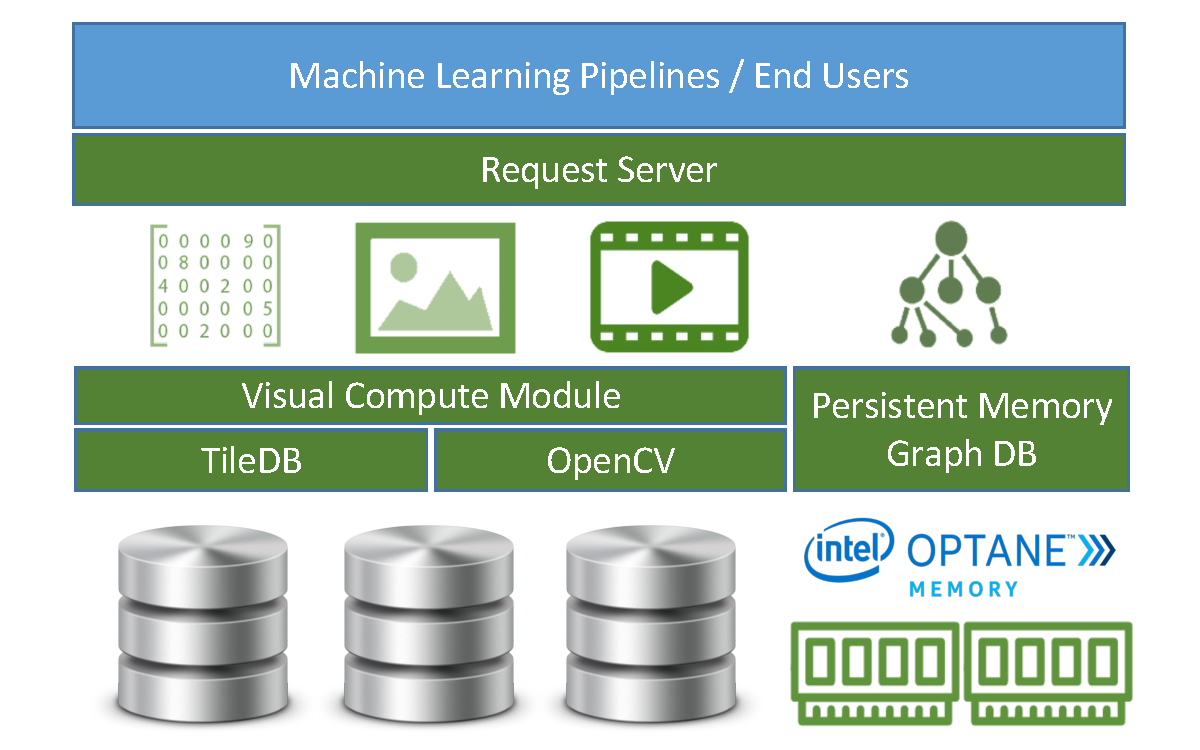
\includegraphics[width=1\columnwidth]{figures/vdms_arch.pdf}
\caption{VDMS Architecture}
\label{fig:arch}
\end{figure}

VDMS implements the typical client-server architecture that handles
client queries transactionally and concurrently, similar to what most common
relational and non-relational database systems
\cite{mysql, postgresql, chang2008bigtable} use.
The main difference between other data management systems and VDMS is that
it goes beyond the typical supported data types (string, integers, floats,
blobs, JSON-documents, etc), recognizing visual entities (image, videos,
feature vectors, etc) as first class citizens.
VDMS API enable users to insert, index, process, and query visual data,
as well as provides full support for inserting, indexing and querying
user-defined metadata.
Users interact with both metadata and visual data using a unified API,
in a transactional manner.

VDMS provides a \textit{graph model} abstraction with the traditional
atomicity, consistency, isolation, and durability
(ACID) properties expected from databases.
This is, users interact with their objects (metadata, images, videos, etc.),
as if these objects were in a connected graph.
Graph represents an easier abstraction to model complex problems,
making it very suitable for the data and access patterns shown by visual metadata,
which can be easily mapped into application-level abstractions by
developers~\cite{tao}.
For instance, abstractions like \textit{BoundingBoxes} associated to
images or videos can be easily represented using nodes and edges in a graph.
This is the main reason why the team chose a graph model over a
relational one for the implementation of VDMS API.

VDMS API provides a mechanism to insert and connect Images, Videos, BoundingBoxes,
Frames, and Descriptors (feature vectors), together with any metadata
associated with the objects.
Each object is a node in the graph.
The information associated to each visual object (image, video, etc.) is modeled as
"properties" of the node in the graph.
Users can query, filter, and retrieve these objects based on its properties.
VDMS does not simply treat these objects as binary blobs of data, but rather
understands them and the type of processing that is common for them,
providing the ability to run processing on-the-fly, both at insertion and
retrieval time. This is one of the main differentiating aspects when compared to other
database systems, including relational databases.
In a relational database, for instance, one can query \textit{and compute}
over values in a column only for basic data types (strings, integers, floats),
and over the abstractions the relational model supports (tables, columns).
This is, a SQL query can retrieve the \textit{computed average} "salary" of all
the employees in a company (stored using the table/columns abstraction),
but cannot perform any computation over data stored as a blob or binary object.
VDMS, because it recognized the nature of visual objects by design,
provides the ability to \textit{compute} on these visual objects
(image, videos, etc.).

VDMS API also allows users to insert application-defined "Entities",
that enable applications to model any use-case specific metadata.
An "Entity" object (and its properties) is a node in the graph.
For example, a user can define an Entity object of a class "Person",
and \textit{connect} this person to one or multiple image objects.
Later, the user can retrieve the Entity object corresponding to a person,
together with all the images \textit{connected} to it. In some cases,
users may need to apply different processing operations to the visual data
for their application. We chose to support
specific operations due to their frequent use in ML applications using
visual data. Common operations supported for both images and videos are
thresholding, cropping, and resizing. Additional operations such as
flipping and rotation are supported for images and extracting
frames by interval is supported for videos.
In most ML applications, a subset of these operations are included in
the preprocessing stage of model training and/or inferencing which supports
majority of the research communities who analyze visual data and may benefit
from replacing customized solutions with VDMS.

By providing the ability to store visual data objects together with
application-defined entities and its properties, VDMS can manage
all the data the application need behind a single, unified API.
This means users can access all data (metadata, images, videos, etc.)
from the VDMS API and even implement their own API/front-end on top
of VDMS without adding any additional abstractions.
This is in contrast with current applications that rely on a combination
of multiple data management systems and APIs to access different
portions of the data they need
\cite{tao, sculley2015hidden, mayer2020scalable, sculley2015hidden}.

Figure \ref{fig:arch} depicts the high-level architecture of VDMS, which
is composed by several sub-components, and a Query Engine that implements
the unified API and hides all the complexity underneath.
We first describe the VDMS API, and then describe its sub-components
and design decisions.

\subsection{VDMS API}

One of the most important differentiating aspects of VDMS is its API.
VDMS is unique in recognizing visual entities (i.e., images, videos, etc.)
as first class citizens.
Thus, VDMS' API revolves around visual data operations and retrieval,
but at the same time, enables applications to store any other
application-specific metadata.
VDMS API is easy to use and explicitly pre-defines certain
primitives associated with metadata, images, videos, and feature vectors.
Authors have paid particular attention to hide the complexities of our internal
implementation and up-level the API to a JSON-based API,
which is very popular across various application domains.
By defining a new JSON-based API, there is a trade-off between expressiveness
(compared to well-established query languages like SPARQL, Gremlim, or even SQL)
and the ability to natively support visual data operations.
However, we believe it is possible for our API to achieve similar levels of
expressiveness compared to more mature query languages over time.

Listing~\ref{addimageandautotag} shows a sample query for inserting
an image, properties associated with the image, and metadata to VDMS.
The metadata, in this case, is the information about the "autotag",
which is provided by the dataset in this specific
\textit{image-search} application.
In this example, the transaction inserts an application-defined "Entity" of
the class "autotag", with the "name" property being \textit{alligator},
inserts an Image with its "latitude" and "longitude",
stores the image as a JPG (VDMS will transcode if needed),
and creates a connection between the Image and the Entity, with a "prob"
property (which indicates the probability of that image
containing an object of type  \textit{alligator}) with a specific value.
This query is performed \textit{transactionally}: either all the image, metadata
and connection are inserted, or none of them are and an error is returned.
Note that no schema needs to be defined in advance.
The Entity of class "autotag", with its properties, are declared and added
at insertion time, without any need to define a schema of objects
(and its properties) before hand. This is a benefit over relational
databases which require the user to identify how data is divided into
different tables and determine the relationship between tables.

\begin{listing}[ht!]
\begin{minted}[frame=single,
              framesep=3mm,
              linenos=true,
              xleftmargin=21pt,
              fontsize=\footnotesize,
              tabsize=4]{js}
"AddEntity"{
    "_ref" : 1,
    "class": "autotag",
    "properties": {
        "name": "alligator"
    }
},
"AddImage":{
    "_ref": 2,
    "properties": {
        "latitude":    36.23433,
        "longitude": -116.80666
    },
    "format": "jpg"
},
"AddConnection": {
    "ref1": 1,
    "ref2": 2,
    "properties": {
        "prob": 0.7653
    }
}

\end{minted}
\caption{Sample Query for Image Insertion -
The query expresses the following:
Insert an Entity of the class "autotag", with the "name" property being
\textit{alligator}, insert an Image with its "latitude" and "longitude",
store the image as a JPG, and create a connection between
the image and the "autotag", with a property "prob"
(which indicates the probability of that image
containing an object of type \textit{alligator}).}
\label{addimageandautotag}
\end{listing}

Listing~\ref{findimagegeo} shows another sample query, in this case, for retrieval.
In this particular example, the transaction retrieves all the images
of \textit{alligators} with probability higher than 0.66,
filter by latitude and longitude within 1 degree,
apply a resize operation to make the images 224x224,
rotate the images 45.34 degrees, and return the images as "png" files.
It is important to note how the API natively supports basic building
blocks of visual data processing, like resize, rotation, or transcoding
(changing output formats and encodings).
Moreover, because VDMS is in control of the metadata and the image data,
re-ordering or pre-processing operations can be done transparently,
increasing the performance of the retrieval process.
The API allows interaction with metadata, images, videos, bounding boxes,
frames, feature vectors, and more in a similar fashion,
and it is fully documented on the project's Github
wiki~\footnote{https://github.com/IntelLabs/vdms/wiki/API-Description}.
The visual data pre-processing operations supported in VDMS are generic and
application independent.
By design, we only include pre-processing operations that are not specific
to one domain, but rather general for visual analytics.



\begin{listing}[ht!]
\begin{minted}[frame=single,
              framesep=3mm,
              linenos=true,
              xleftmargin=21pt,
              fontsize=\footnotesize,
              tabsize=4]{js}
"FindEntity"{
    "_ref" : 1,
    "class": "autotag",
    "constraints": {
        "name": ["==", "alligator"]
    }
},
"FindImage":{
    "format": "png",
    "constraints": {
        "latitude": [">=", 36.23433,
                     "<=", 38.23433]
        "longitude":[">=", -114.80666,
                     "<=", -116.80666]
    },
    "operations": [{
            "type": "resize",
            "height": 224,
            "width":  224,
        }, {
            "type": "rotate",
            "angle": 45.34
    }],
    "link": {
        "ref":1,
        "constraints": {
            "prob": [">=", 0.66]
        }
    }
}

\end{minted}
\caption{Sample Query for Image Retrieval -
The query expresses the following:
Find all the images connected to the autotag \textit{alligator}
with probability higher than 0.66,
filter the images by latitude and longitude within 1 degree,
apply a resize operation to make the images 224x224,
rotate the image 45.34 degrees,
and return the images as "png" files.}
\label{findimagegeo}
\end{listing}

\subsection{Graph Engine}

The Graph Engine used in VDMS is the
\textit{Persistent Memory Graph Database} (PMGD).
PMGD was developed at Intel Labs, and was designed and optimized for
persistent memory technologies like Intel Optane~\cite{IntelXPoint15}, which
promise storage providing nearly the speed of DRAM and the
durability of block-oriented storage.
PMGD is also fully open-sourced \footnote{https://github.com/IntelLabs/pmgd}.
PMGD implements an in-persistent-memory graph database optimized
to run on a platform equipped with persistent memory, but
also provides the option to run on SSD and ext4 filesystem
using OS support to provide transactional guarantees (through \textit{msync}).
PMGD provides a property graph model of data storage with the traditional
atomicity, consistency, isolation, and durability
(ACID) properties expected from databases.
Specifically, the database remains consistent, each transaction either
completes entirely or not at all, and the effects of a completed transaction
survives any failure.
In cases where the system may crash or fail, PMGD has the ability
to recover to a consistent state without loading its content into memory.
Unlike existing graph databases that are disk-based, our graph engine
avoids converting data from a disk-friendly format to an usable format for an application.
PMGD comes as a C++ library that VDMS uses for implementing its query engine.
Because PMGD already supports most of the graph abstractions we wanted
to see on VDMS API, it was our preferred option.
Also, our internal evaluation shows that PMGD is faster
than other graph databases, including Neo4j\cite{miller2013graph}.
In this paper, the evaluation uses SSDs instead of persistent memory.
Hence, PMGD performance evaluation will be published separately to highlight
the advantages of using persistent memory for visual data.

\subsection{Visual Compute Module}

% The Visual Compute Module enables machine-friendly enhancements to
% visual data, exposing high-level abstractions to the \textit{Request Server}
% for dealing with a variety of images and video formats (through OpenCV and ffmpeg),
% and different methods for indexing for feature vectors
% (including Facebook's Faiss \cite{faiss}, TileDB \cite{TileDB}).
% Finally, a main component of VDMS is in charge of implementing the
% API and orchestrating between the PMGD and the Visual Compute Module
% to serve client's requests. This component is the \textit{Request Server}.

The Visual Compute Module was designed and implemented to provide
an internal abstraction layer for interacting with visual data.
It enables the query engines to coordinate and perform
visual data handling and processing
(i.e., basic building block operations like crop, resize, etc. for images/videos
and k-nearest neighbor search for feature vectors),
shown in Figure \ref{fig:arch}.
For traditional formats (jpg, png, tiff, mp4, etc.),
the interface is an abstraction layer over OpenCV.
However, it also provides a way to use novel formats that are
better suited for visual analytics: a novel, array-based lossless image format.
This format is built on the array data manager TileDB~\cite{TileDB} and
is well suited for images that are used in visual analytics.
Note that, even if VDMS currently provides support for array-based lossless
image format, we do not use it as part of this evaluation.
This work focuses on a more direct comparison with a combination of alternatives,
and thus we use the traditional format (jpg and png).
The performance comparison between the array-based lossless image format
we developed and other similar formats (like png or tiff) are outside of the
scope of this evaluation.

VDMS also provides full support for video storage and operations,
in a similar way it does for images.
This includes support for encoding, decoding, and transcoding of
\textit{mp4}, \textit{avi}, and \textit{mov} containers,
as well as support for \textit{xvid}, \textit{H.263} and \textit{H.264} encoders.
This is supported through the use of either OpenCV~\cite{opencv}
or \textit{libffmpeg}\cite{ffmpeg}, or both,
plus additional implementation to support fast random access to video frames.
All operations supported for images in VDMS are also supported at the
video and frame level of the API.
On top of that, there are a number of video-specific operations that
are supported, such as the interval operations,
enabling users to retrieve clips at different
frames-per-second (fps) versions of the video.

Another key differentiating factor of VDMS is that it allows the creation of
indexes for high-dimensional feature vectors and the insertion of
these feature vectors associated with entities, images, and/or videos.
Feature vectors are intermediate results of various machine
learning or computer vision algorithms when run on visual data.
Feature vectors are also known as \textit{descriptors}
or \textit{visual descriptors}.
We use these terms interchangeably.
These descriptors can be classified, labeled, and used to build search indexes.
Feature Vectors support is provided through our implementation based
on high-dimensional sparse arrays, also using array-based approaches.
In addition, the Visual Compute Library provides a wrapper
for another high-dimensional index implementation,
Facebook's Faiss~\cite{faiss}.
Users can, through our API, use different indexing techniques
for feature vectors, depending on their application's need.


\subsection{Client Library}

The client library implements TCP/IP based connectors to the VDMS Server,
similar to most databases\cite{memsql, mysql, postgresql}.
Users can connect to VDMS and run queries using VDMS' API
by defining a transaction using JSON objects.
The client library provides a simple method that
accepts a JSON string and an array or vector of blobs.
Internally, the library wraps the query string and blobs using
Google Protobufs \cite{protobufs} and sends it to the VDMS server.
It also receives a similarly formed response from VDMS
and returns it to the client.
Currently, client libraries are implemented for Python and C++ client.
The client libraries are lightweight, as they simply implement the communication
protocol between the client and the server.
This makes it easier for developers to implement similar client libraries using
any other programming language of their choice.

\section{Evaluation}
\label{eval}

We have used the YFCC100M dataset to evaluate different aspects of our system.
We use the images in the dataset and its associated metadata to implement
an image-search engine based on properties associated with those images.
This is a very common use-case we have encountered when building
applications such as smart-retail, sports applications, and video summarization.
For these type of applications, the starting point is usually
a large set of data that must be curated
before proceeding with the data processing (such as neural network training).
In order to evaluate the different aspects of the performance on the
image search, we have built different baselines following the methodology
used in the industry, and following what we have done in the past
in order to solve the data search problem,
which we describe in Section \ref{images}.
% We have also included performance evaluation on the Video and Feature Vectors
% functionality in the appendix for further reference, together with a
% description of the key aspects of those functionalities.

\begin{figure*}
\centering
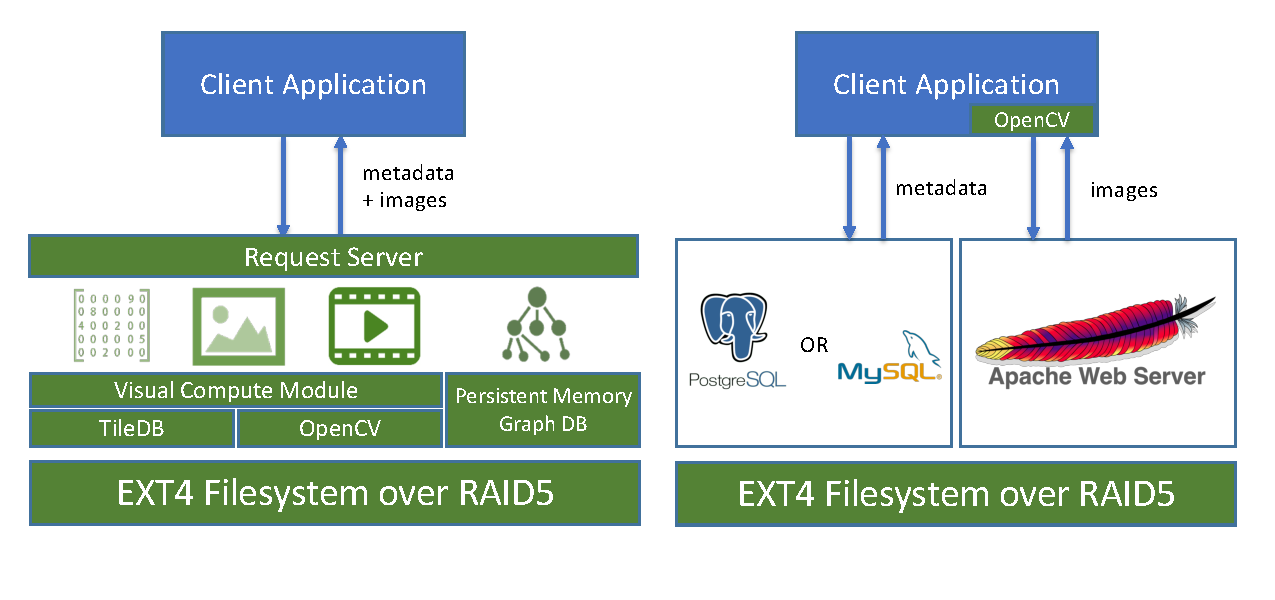
\includegraphics[width=\textwidth]{figures/comparison_system}
\caption{Comparison Systems: Logical view of the interaction between the client application with VDMS (left) and the baseline systems (right). The baseline systems are either based on MySQL or PostgreSQL for operating and querying metadata.}
\label{fig:systems}
\end{figure*}

\subsection{YFCC100M Dataset}
\label{dataset}

The Yahoo! Flickr Creative Commons 100m (YFCC100M) dataset is a large
collection of 100 million public Flickr media objects created to provide free,
shareable multimedia data for research.
This dataset contains approximately 99.2 million images and 0.8 million videos
with metadata characterized by 25 fields such as the unique identifier, userid,
date the media was taken/uploaded, location in longitude/latitude coordinates,
device type the media was captured, URL to download the media object,
and the Creative Commons license type information.
The YFCC100M dataset also contains \textit{autotags}
provided as a set of comma-separated concepts such as people, scenery, objects,
and animals from 1,570 trained machine learning classifiers ~\cite{Thomee_2016}.
Together with each \textit{autotags}, there is a probability associated with
each tag to indicate certainty of the classification.
This is, an image can have the \textit{autotags} "people", "person", "party",
"outdoor", and each \textit{autotag} assigned will be accompanied by a
probability of that \textit{autotags} being present in that image/frame.
We have also used feature vectors generated for every image and first frame
of every video \cite{features} to implement a similarity search.
Given that there is no standard benchmark oriented towards visual data queries,
we have built a series of queries to filter this dataset that is modeled after
our internal use cases for many of the mentioned applications we have worked
with.

\subsection{Experimental Setup}
\label{setup}

Given that there are no other open-source systems that provide similar
functionality and interfaces as VDMS, we have implemented two equivalent
visual data management system as baselines, comprised of a combination of
widely available, off-the-shelf components.
The first baseline uses MySQL Server 5.7 (for storing metadata),
Apache Web Server 2.4.18 (as interface for image access), and
OpenCV 3.3 (to provide pre-processing operations on images).
The other baseline system replaces the MySQL Server 5.7 with the
most advanced open source relational database, PostgreSQL 9.5 \cite{postgresql}.
We decided to use relational databases in the baseline systems instead of
non-relational databases because~\cite{Jatana2012, li_2019}:

\begin{itemize}
    \item Relational databases support atomicity, consistency, isolation,
    and durability (ACID) while non-relational may compromise some ACID properties.
    \item The YFCC100m data is clearly structured.
    \item We need to efficiently collate and return metadata records.
\end{itemize}

The baseline implementations only partially replicate the functionalities
that VDMS offers when it comes to image and metadata handling, and it was
built for the purpose of an ad-hoc image search implementation.
The baseline implementations are based upon internal tools used for ML-based
pipelines for media, the common practice in the industry \cite{haystack, tao}.
We have implemented a set of client-side applications that take care
of retrieving the components from the different systems, and applies
pre-processing operations when needed.

For all our experiments, we use two servers with Ubuntu 20.04,
one hosting a VDMS server and another hosting the baseline implementations.
Both servers have a dual-socket Intel\textsuperscript{\textregistered}
Xeon\textsuperscript{\textregistered} Platinum 8180 CPU @ 2.50GHz (Skylake),
each CPU with 28 physical cores with hyper-threading enabled,
for a total of 112 logical cores per server.
The server hosting MySQL and PostgreSQL has 256GB of DDR4 DRAM,
while the server hosting VDMS has 194GB of DDR4 DRAM.
We decided to run the VDMS server in the machine with less DRAM to make
sure MySQL and PostgreSQL had no disadvantage, and because previous evaluation
indicated smaller footprint in the case of VDMS when
compared to similar baselines based on MySQL.
To build both MySQL and PostgreSQL on the same machine,
we stored each relational database on separate SSD drives.
Other than the difference in DRAM space and storage needed for two baselines,
the machines are identical.
The client application running the queries and measuring round-trip time
is connected to the server through a 1GB wired link through
a 10GB back-plane switch, same as both servers.
The client application was implemented using Python 3 for both VDMS and the baselines.
Figure~\ref{fig:systems} shows a logical view of the difference between the
interaction of the client application (retrieves metadata and
images) with VDMS (left) and the MySQL/PostgreSQL baselines (right).

It is worth noting that the images are stored in a shared repository
(ext4 filesystem on a RAID 6 configuration of 16TB) that both
Apache WebServer and VDMS have direct access.
In the case of videos, only the first frame is used for the image search.
% More information and evaluation on video-specific functionalities can be found
% in the appendix of this work.
In the case of the baselines, metadata is
stored in MySQL and PostgreSQL using an attached SSD disk.
Even if VDMS has native support for Optane Persistent Memory,
we do not use it in this experiment because of fairness of
comparison with respect to MySQL and PostgreSQL, which were not designed for
Persistent Memory type of storage.
The benefits of Persistent Memory for metadata and a full evaluation of
the PMGD subsystem is material for another paper,
and outside the scope of this evaluation.
For this experiment, in the case of VDMS we simply use a similar
attached SSD disk to store metadata.
Even if PMGD, the graph database used by VDMS, is designed for persistent memory,
it can deliver good performance when using SSDs directly, while still
providing ACID-compliant transactions.

For the metadata, we built VDMS, MySQL, and PostgreSQL databases
using the YFCC100M dataset with incremental database sizes.
For simplicity, we named the database based on the approximate number of images
it contains, as follows: 1M, 5M, 10M, 50M, 100M.
The databases have comparable number of elements.
The exact number of images/elements in each database are shown in
Table \ref{table:vdmsnodes} and \ref{table:mysqltables}.
The differences can be attributed to minor failures in data
preparation/loading because of incomplete/inconsistent formatting,
which is common in large datasets \cite{failures}.
In our set up, that difference is very small: less than 0.253\% in terms of
number of elements (images and/or metadata information).

\subsubsection{Data Representation}


\textbf{VDMS:}
For each database size, we created an instance of VDMS using the image/video metadata,
the machine-generated \textit{autotags} associated with
each image/video identifier, and the list of 1,570 \textit{autotags}.
Internally, that information is represented as a property graph,
where we have one node for each image, one node for each tag
(always 1,570 tags), and a connection between each image and its respective tag(s).
For instance, if an image has four \textit{autotags} assigned,
there will be four connections between that image and
the different nodes for those \textit{autotags}.
The probability the \textit{autotag} is present in an image
is expressed as a property in the \textit{connection} between the two nodes.
Figure~\ref{fig:graph_representation} shows an example on two images,
two \textit{autotags}, and the \textit{connections} between
those \textit{autotags} and the images.
Image id 23143252 has two \textit{autotags} assigned:
\textit{Alligator} with probability 0.285, and \textit{Lake} with probability 0.872.
Image id 86756231, on the other hand, has a single \textit{autotags} assigned:
\textit{Alligator} with probability 0.894.
On average there are 8 tags assigned to each image so
there will be around 8 times more connections than images, as shown
in Table~\ref{table:vdmsnodes}.
Also, each image node will contain multiple properties associated
with it (some of which are listed in Section \ref{dataset}).
% Using the Python Client Module, we insert 1,570 nodes for the \textit{autotags},
% and then insert nodes for the YFCC media objects (images or videos)
% with the associated metadata (as properties of the image/video).
% Then, for each image, we add a \textit{connection} between the image node
% and the \textit{autotag} node. The probability of that \textit{autotag}
% being present in that image is stored as a property in that \textit{connection}.
The number of nodes (representing images and \textit{autotags})
are dependent on the database size and the \textit{connections} are responsible for
90\% of the elements in each database instance,
as shown in Table~\ref{table:vdmsnodes}.
It is also important to note that we create indexes for the image identifier,
\textit{autotags} properties, and longitude/latitude coordinates
to enable faster retrieval.

\begin{figure}[ht]
\centering
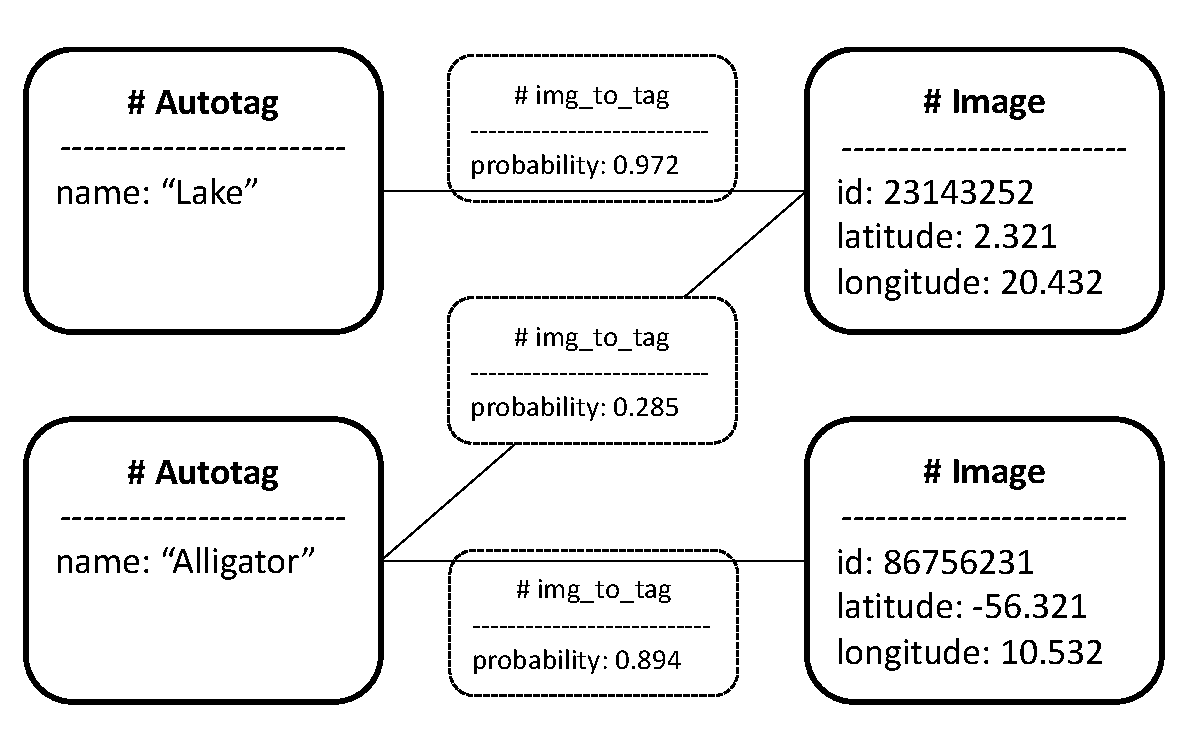
\includegraphics[width=\columnwidth]{figures/graph_representation}
\caption{VDMS Data Representation Using a Property Graph:
Example on two images and 2 \textit{autotags} with
their respective probabilities expressed in the \textit{connection}.
Image id 23143252 has two \textit{autotags} assigned:
\textit{Alligator} with probability 0.285, and \textit{Lake} with probability 0.872.
Similarly, Image id 86756231 has a single \textit{autotags} assigned:
\textit{Alligator} with probability 0.894.}
\label{fig:graph_representation}
\end{figure}

\begin{table}[ht]
\caption{VDMS Database - Number of Elements}
\centering
\begin{tabular}{c c c c}
\hline\hline
DB Name & \# Images & \# Connections & \# TagList\\
\hline
% 100k & 100,000     & 848,432      & 1,570\\
% 500k & 500,000     & 4,249,500    & 1,570\\
1M   & 1,000,000   & 8,503,045    & 1,570\\
5M   & 5,000,000   & 42,505,478   & 1,570\\
10M  & 10,000,000  & 85,040,404   & 1,570\\
50M  & 50,000,000  & 425,162,070  & 1,570\\
100M & 99,205,984  & 895,572,430  & 1,570\\
\hline
\end{tabular}
\label{table:vdmsnodes}
\end{table}

\textbf{MySQL/Baseline 1:}
Each MySQL database is created in a similar manner as VDMS
but the data is represented as three tables, following the relational model:
1) \textit{images} table: contains one row per image,
and a column for each property
associated with the images (some of which are listed in Section \ref{dataset});
2) \textit{taglist} table: contains one row per autotag element
(always 1,570 rows);
3) \textit{autotags} table: contains one row per autotag
assigned to an image. Each row contains a foreign key to the
image, a foreign key to the tag, and
the probability assigned to that tag belonging to that image.
Given that there are 8 autotags, on average, per image, the \textit{autotags}
table has around 8 times the number of rows present in the
\textit{metadata} table, as can be seen in Table~\ref{table:mysqltables}.
Using a Python client and simple queries, the \textit{taglist}
table is read from the list of tags with an auto-incremented
\textit{tagid} as a primary key, and the metadata table
is read from the YFCC100M metadata using the identifier as a primary key.
The \textit{autotags} table contains the generated autotags and
probabilities for entries of the \textit{images} table.
To generate the table, we split the \textit{autotags} data for each database
by the image identifier and autotag into new files.
The new files are read into the \textit{autotags} table with the image
identifier and \textit{tagid} as foreign keys.

In an attempt to have the best MySQL configuration possible for this use case,
we explore several parameters to increase the performance
of both loading the data, as well as executing the queries.
In particular, MySQL optimizes threads and transactions out-of-box,
but it cannot handle the entire YFCC100M dataset without configuring
specific parameters.
When creating large databases, a data lock may occur to protect the
data from concurrent updates~\cite{mysql_blog}.
To avoid this mechanism, we increased the buffer pool size to
increase the amount of memory allocated to internal data structures.
It is recommended to set the buffer pool size to 60-80\% of the physical
memory size ~\cite{mysql,mysql_blog}.
However, the time to build a database increased.
We later changed  the buffer pool size to a multiple of the default value, i.e. 16x,
which produced the best results for loading time.

By default, MySQL uses the available operating system threads to
execute \textit{n} requests in parallel where \textit{n} is
the number of background read/write I/O threads.
Setting the respective parameters in the MySQL configuration file can limit the
number of concurrent threads and the number of background threads.
When a limit is set on the number of threads, and no threads are available,
requests will go into a FIFO queue until threads are available to execute
the request ~\cite{mysql,mysql_blog}.
We ran a few experiments investigating the effects of setting a limitation on the
number of concurrent and background threads.
We concluded that the default settings perform better for large databases instead of
setting a limit.
Therefore, we let MySQL automatically handle the concurrency.

\textbf{PostgreSQL (Baseline 2):}
Each PostgreSQL database is created in the exact same manner as MySQL
where data is represented as three tables:
\textit{images}, \textit{taglist}, and \textit{taglist}.
PostgreSQL works well out-of-box and optimizations were not necessary,
as in MySQL, to load or execute queries.
When executing queries for larger databases,
it is pertinent to have enough disk space for both
the database and tablespace.
The tablespace is associated with a database and stores the temporary files
created within the database object ~\cite{postgresql}.
When processing the larger databases, additional
storage may be needed for the tablespace or a diskfull error may occur.
To avoid this, we allocated a separate SSD disk specifically
for the tablespace of all databases.

By default, PostgreSQL can manage concurrent access to data well using
Multiversion Concurrency Control (MVCC) and a Serializable Snapshot Isolation
(SSI) level of transaction isolation.
MVCC provides better performance by using SSI to guarantee querying data never
blocks writing data, and vice versa ~\cite{postgresql}.
The PostgreSQL configuration file initially limits the maximum
number of concurrent connections to the database server to 100.
We increased this limit to 200 to complete the concurrency analysis
in Section \ref{concurrency_analysis}.

In the case of VDMS, we did not attempt to tune any
parameter to avoid unfairness in the comparison against the baselines.
Unlike the baselines, VDMS can handle the entire YFCC100m dataset
using the default parameters provided by the implementation.
For all systems, we created indexes over the
properties we used for search, such as name of
\textit{autotag}, and geo-location values.
Building indexes for the right properties and objects
is basic operation that would be present in any real-world deployment,
and measuring performance without them would lead to useless analysis in our
real-world applications and use cases.

\begin{table}[ht]
\caption{MySQL and PostgreSQL Databases - Number of Rows in each Table}
\centering
\begin{tabular}{c c c c}
\hline\hline
 & \multicolumn{3}{c}{Table}\\
\cline{2-4}
DB Name & images & autotags & taglist\\
\hline
% 100k & 100,000    & 848,912     & 1,570\\
% 500k & 498,707    & 4,241,200   & 1,570\\
1M   & 1,000,000  & 8,508,380   & 1,570\\
5M   & 4,987,379  & 42,425,905  & 1,570\\
10M  & 10,000,000 & 85,095,265  & 1,570\\
50M  & 50,000,000 & 425,446,208 & 1,570\\
100M & 99,206,564 & 896,002,496 & 1,570\\
\hline
\end{tabular}
\label{table:mysqltables}
\end{table}

% \begin{figure}[ht]
% \centering
% 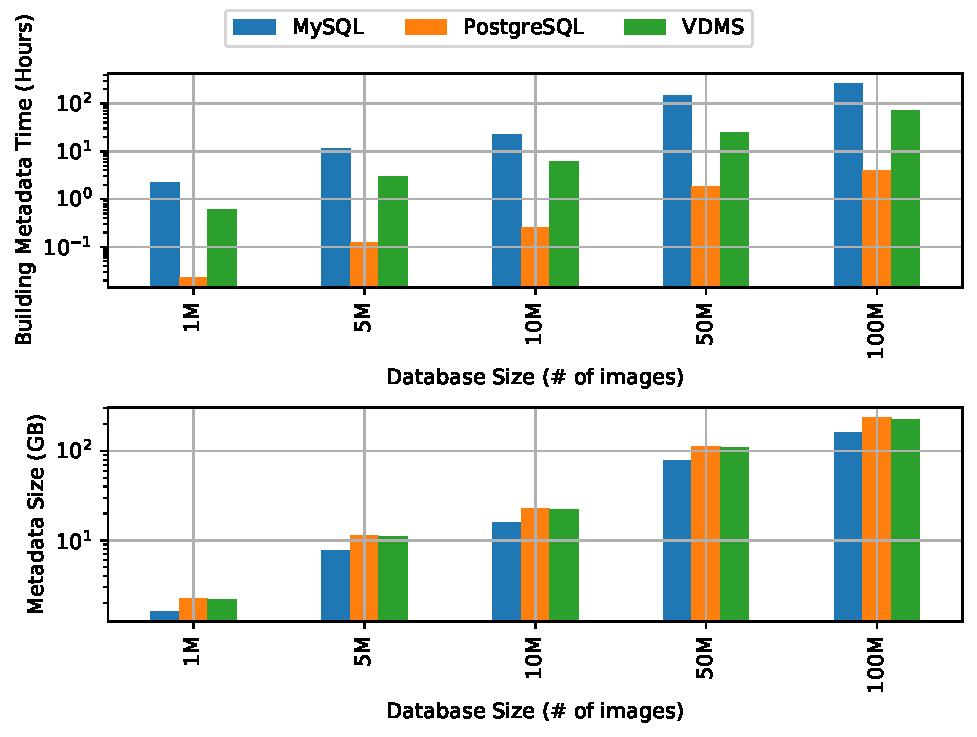
\includegraphics[width=\columnwidth]{figures/all_build_times_plot}
% \caption{Time to build and size (in GB) of MySQL, PostgreSQL, and VDMS databases.}
% \label{fig:db_time_size}
% \end{figure}

\begin{figure}[ht]
\centering
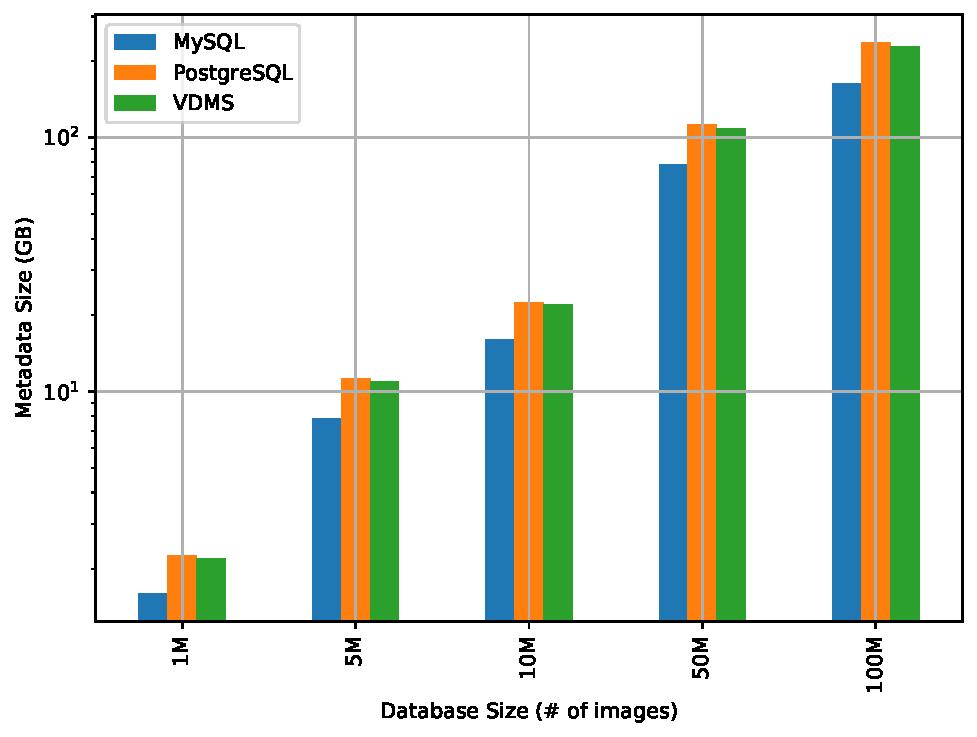
\includegraphics[width=\columnwidth]{figures/all_build_sizes_plot}
\caption{Data footprint (in GB) of MySQL, PostgreSQL, and VDMS databases.}
\label{fig:db_sizes}
\end{figure}

% \subsubsection{Database Building Time}

% One of the first things we noticed is the difference in the time needed to
% build each database, where VDMS outperforms MySQL by a large margin
% but PostgreSQL outperforms VDMS by a large margin as well.
% This analysis includes only the metadata, as the images are stored
% in a shared filesystem. Figure~\ref{fig:db_time_size} illustrates the
% comparison in time to build the databases, and how the speedup
% is sustained as the database size grows.
% Key difference in the build times are attributed to the low-level
% implementation of how MySQL reads and stores data from the files, the
% optimizations (increased InnoDB pool size, etc.) needed
% to handle large datasets such as YFCC100M, and the efficiency of PMGD.
% PostgreSQL Python API can efficiently copy data from files to the database
% which provides an advantage over VDMS which must insert
% multiple nodes/connections per image.
% On average, it took MySQL around $\sim$4x longer to build each database than VDMS,
% and PostgreSQL was around $\sim$21x faster than VDMS.

\subsubsection{Database Storage Footprint}

% Another important aspect to note is the storage footprint of the databases.
PostgreSQL and VDMS require comparable amount of storage for metadata which
is more than required by MySQL, shown in Figure~\ref{fig:db_sizes}.
In the case of VDMS, this is space used to store information about
each node/connection.
The Graph Database internal to VDMS (called PMGD) was designed for performance,
especially in environments where persistent memory is present.
This design decision comes as a trade-off for storage footprint, which is
noticeable in our results.
VDMS required 37-41\% more storage than MySQL for storing the same amount
of metadata. On the other hand, PostgreSQL required 1-4\% more storage than VDMS.
The storage footprint may become a factor if storage is a limitation, but
it should also be noted that metadata accounts for less than 2\% of the
overall database size even if we have a 41\% increase in metadata size.
For example, the largest database (both metadata and images) we built
(100M) has around 230GB of metadata and 12TB of images.
In systems where persistent memory is a scarce resource,
the increased storage foot print of PMGD may represent a challenge.
On the other hand, persistent memory is expected to be available
in the order of TBs per server, which should fit the
metadata of intensive use-cases\cite{IntelXPoint15}.

%=========================================

\subsection{Images Search}
\label{images}

In order to evaluate VDMS and the baseline systems on our use-case queries,
we implemented 6 queries that filter and retrieve a specific set of images.
We chose these queries because they represent typical use-cases where a
cohort of images is to be retrieved and processed from a large corpus of data.
As we mentioned before, we took this approach mainly because we wanted to
replicate systems we have built internally for our use cases,
and also because of the lack of standard
benchmarks that are oriented towards visual data retrieval.

We use the metadata associated with the images to filter the images.
We use the \textit{autotags} (as they contain information about the content
of the image), and geo-location information (latitude/longitude)
of the images for search and filtering.
Note that, even if we use geo-location for our study, any other property
assigned to the images can be used to refine the search
in both VDMS and baseline implementations.
On top of that, and for our use cases, we would like to extract more information
about the content of the image through the use of ML,
such as Convolutional Neural Networks~\cite{cnn}.
For this, we resize the images to 224x224, which is the input layer size for
popular variations of neural networks for object detection on images~\cite{resnet}.
We used both ResNet and Yolov3 for object detection, both of which
have the requirement of a downsized, lower resolution image as input.

To evaluate the access to metadata and images,
we use the following queries, modeled after our internal use cases:

\begin{itemize}
\item \textit{q1} - {\bf {\em 1tag\_resize}}: Retrieve images with one specific autotag and resize to 224x224.

\item \textit{q2} - {\bf {\em 1tag\_geo\_resize}}: Retrieve images with one specific autotag, in a particular geo-location, and resize to 224x224,.

\item \textit{q3} - {\bf {\em 2tag\_and\_resize}}: Retrieve images with two specific autotags (i.e. alligator AND lake), and resize to 224x224.

\item \textit{q4} - {\bf {\em 2tag\_or\_resize}}: Retrieve images with either of two specific autotags (i.e. alligator OR lake), and resize to 224x224.

\item \textit{q5} - {\bf {\em 2tag\_resize\_geo\_and}}: Retrieve images with two specific autotags (i.e. alligator AND lake), in a particular geo-location, and resize to 224x224.

\item \textit{q6} - {\bf {\em 2tag\_resize\_geo\_or}}: Retrieve images with either of two specific autotags (i.e. alligator OR lake), in a particular geo-location, and resize to 224x224.

\end{itemize}

It is important to note that when querying for images with certain
\textit{autotags}, we also apply a filter using the probability.
For instance, we only retrieve images with an autotag \textit{alligator}
and a probability higher than 92\%.
These probabilities are both present in VDMS (in the form of a property
of the \textit{connection} between the image and that \textit{autotag}),
as well as in MySQL and PostgreSQL (in the form of a column in the
\textit{autotags} table that links images with tags).
In the case of VDMS, the query involves a graph traversal query that starts
from the \textit{autotag} node and ends in the images node,
following \textit{connections} between the image and that \textit{autotag}).
In the case of the baseline implementations,
the query involves JOIN operations between the 3 tables.
The implementation of this evaluation, as well as all the queries, are available
under the benchmarks branch of the VDMS project
\footnote{https://github.com/luisremis/visual\_storm/tree/master/yfcc100m},
and some examples of the queries can be found in the appendix of this paper.

Also, note that the size of the result (number of images retrieved)
is linear with the size of the database. This is, if a query returns 100 images
for the 1M database, it will return around 1000 images for the 10M database.
This poses a problem when evaluating performance as the size of the database increase,
and clearly understanding the measurements.
Because of this reason, we control the number of returned images for all the
databases using the probability of the \textit{autotags}
(higher probabilities returns less images), so that the queries in
this experiment return a similar number of images for all database sizes.
In other words, as the size of the database increase, we increase the probability
threshold for the queries. We do this for both VDMS and the baselines, of course.
This way, we remove bottleneck introduced by network bandwidth that would
otherwise over-complicate the understanding of the results.

Image search based on metadata is very expensive in large databases.
Because of the large volume of data, the processing of the retrieved images
is performed in parallel, using multi-core and/or distributed systems.
For instance, a common implementation of an image processing pipeline
would involve the use of distributed processing frameworks
like Hadoop \cite{hadoop} or Spark \cite{spark}.
Consequently, it is key that the data management system used supports
concurrency, providing multiple workers with data in parallel.
The ability to scale with the number of simultaneous clients is key for the
applicability of visual data management systems like VDMS.
Because of this, we put emphasis on the analysis of concurrency and throughput,
rather than latency.


%% ========= Concurrency Comparison Analysis

\subsubsection{Concurrency Analysis} \label{concurrency_analysis}

\begin{figure}[ht]
% WAS: begin{figure*}[ht]; textwidth
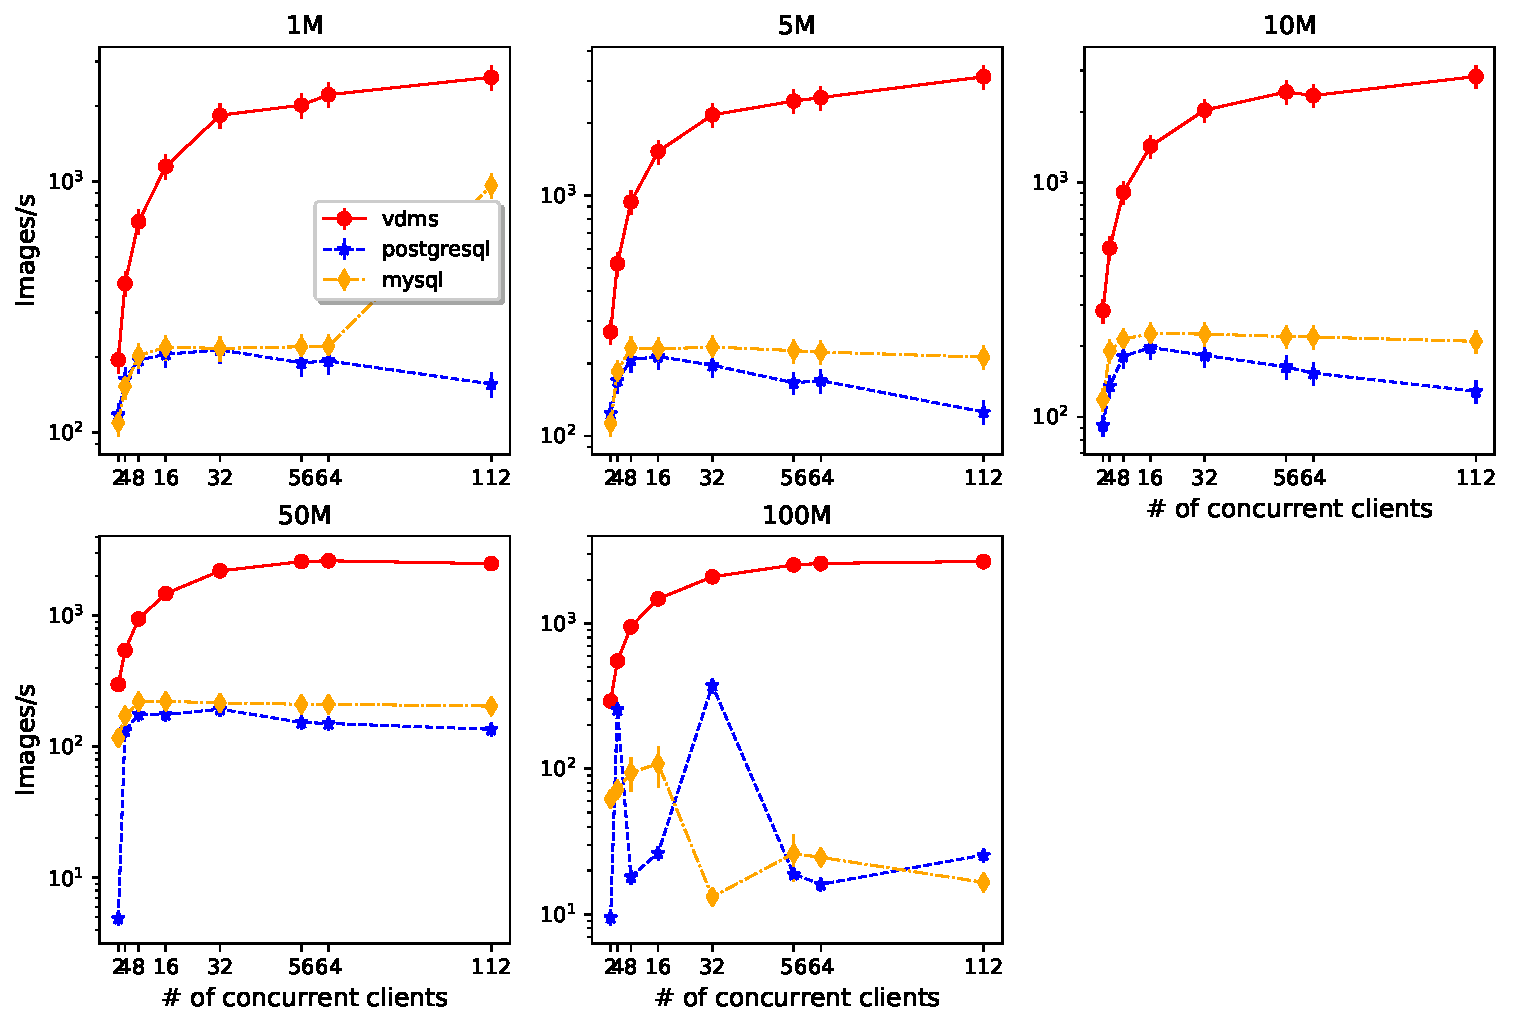
\includegraphics[width=\columnwidth]{figures/plot_conc_q_1tag_geo_resize_mosaic_results_throughput_db_size}
\caption{Concurrency Analysis on \textit{q2} (\textit{1tag\_geo\_resize}) from our use-case
described in the Experimental Setup Section.
We show each database in different figures for readability reasons.
The figures show the throughput (images per second) when retrieving
resized versions of the images, as the number of concurrent clients increases
Hardware concurrency (number of physical cores in each system)
is shown with a blue vertical line (hw-concurrency = 56).}
\label{fig:concurrency_comparison_q2}
\end{figure}

Figure~\ref{fig:concurrency_comparison_q2} illustrates a concurrency analysis for
\textit{q2} (\textit{1tag\_geo\_resize}), described above,
using VDMS and the baselines.
Here we evaluate the scalability of all systems, as the number of concurrent
clients grows (x-axis) and as the size of the databases grow.
Figure~\ref{fig:concurrency_comparison_q2} shows throughput (images per second)
when retrieving resized versions of the images, as the number of
concurrent clients increase.
The first thing to notice is that VDMS outperforms both baselines for all
databases for this query by a large margin.
For the baseline systems, in the case of 100M, the increase in the
size of data seems to have a larger impact in performance.
This result can be attributed to the increase in the complexity of the JOIN
operation as the number of rows in the tables increases.

Another thing to notice is that, as the number of concurrent clients increases,
VDMS throughput continues to increase up to 56 threads, which is
the hardware concurrency of the system.
Also, more parallelism after 56 threads does not increase the delivered throughput
for the larger databases (50M and 100M) but there is a slight improvement in the
other databases (1M, 5M, and 10M).
On the other hand, both baselines seem to deliver less aggregated
throughput after 16 threads except for the 100M case.
In this case, PostgreSQL has a performance spike at 32 clients
and the performance for both baselines is less stable when compared
to VDMS.
Note that most of the throughput for the baseline systems are very close to each other.
This is mostly an effect of the log-scale used, which is needed to clearly
depict the difference between VDMS and the baselines.
Here, the baselines are the full architecture described in
Figure~\ref{fig:systems} (right).

All queries run a resize operation on the image,
an operation that requires decoding, resizing, and encoding the image
before sending it back to the client.
These operations are mainly compute bound, and that is the reason for
the system to stop scaling beyond the number of physical cores.
In contrast, the baseline does not scale nearly as well as VDMS,
and we see that even after increasing concurrency, the increase
in throughput is just about 2x.
When comparing the case of 56 or 64 concurrent clients,
VDMS delivers between 8x and 10X the throughput.

\begin{figure}[ht]
% WAS: begin{figure*}[ht]; textwidth
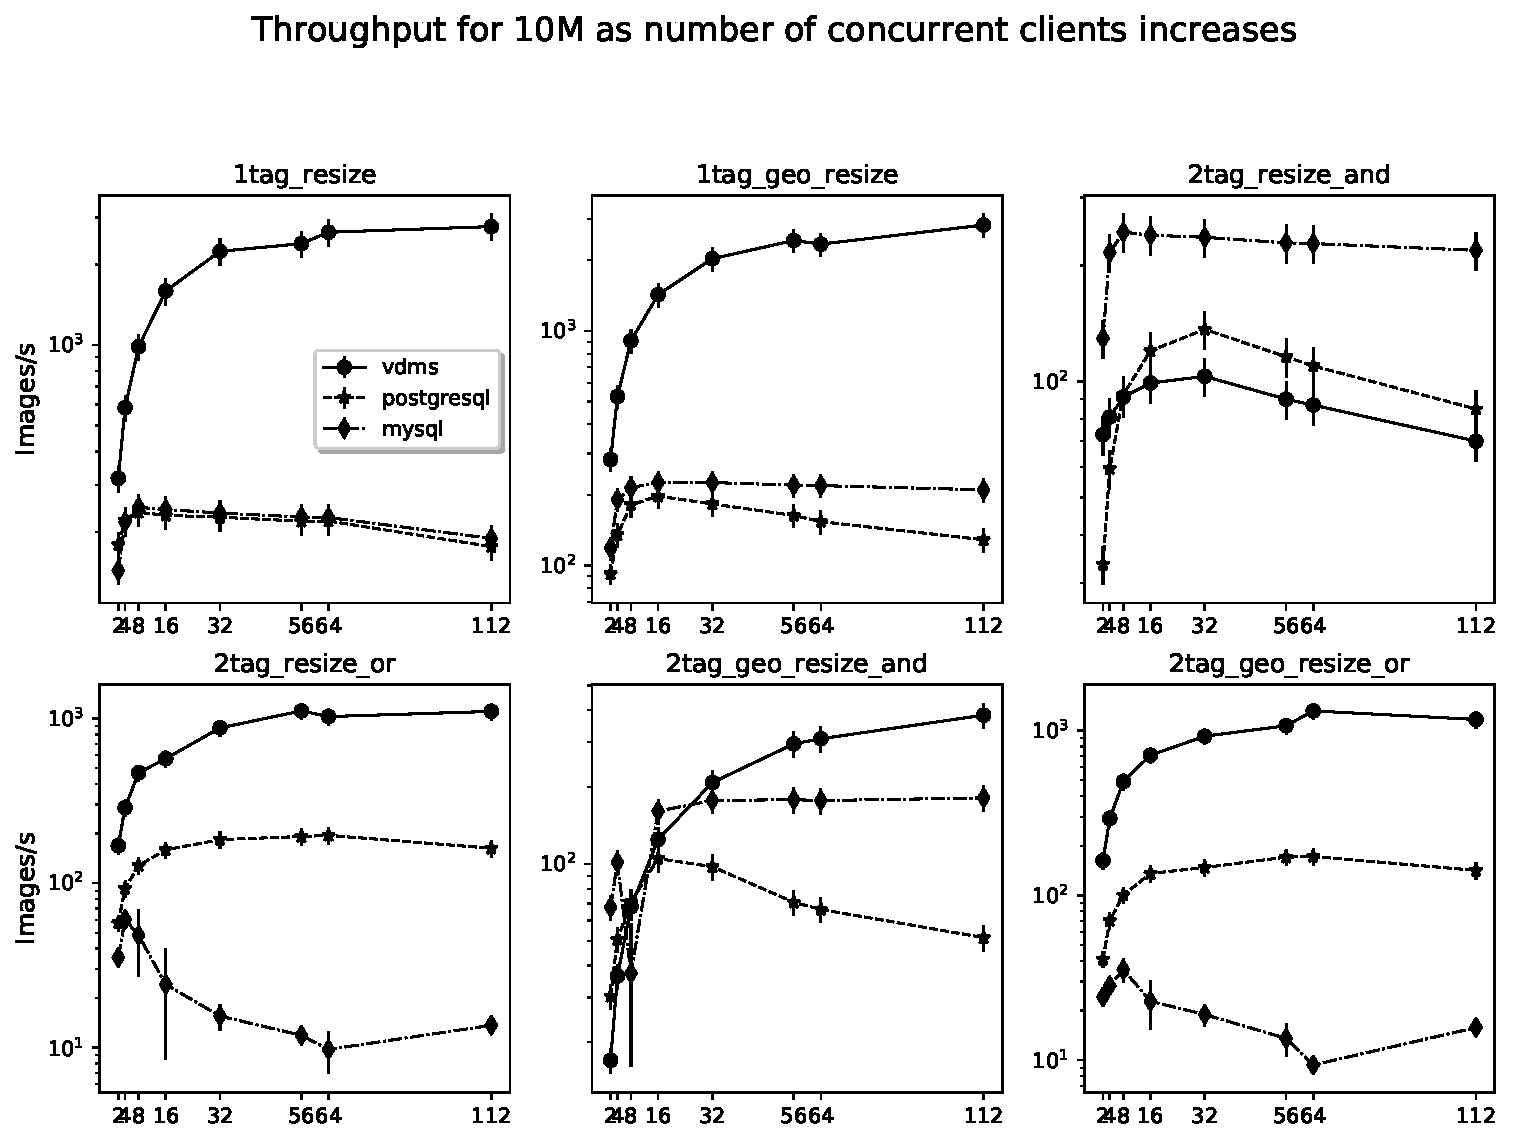
\includegraphics[width=\columnwidth]{figures/plot_conc_dbsize_10M_mosaic_results_throughput}
\caption{Concurrency Analysis for all the queries using the 10M database).
We show queries in different figures for readability reasons.
Each figure shows the throughput (images per second) when retrieving
resized versions of the images as the number of concurrent clients increases.
Hardware concurrency (number of physical cores in each system)
is shown with a blue vertical line (hw-concurrency = 56).}
\label{fig:concurrency_comparison_10M}
\end{figure}

We continue by looking at Figure~\ref{fig:concurrency_comparison_10M}
which shows the images per second delivered by each system
for all queries using the 10M database, as the number of concurrent
clients grows (x-axis). This figure takes a closer look at the
concurrency for each of the six queries.
It is obvious that VDMS consistently outperforms each of the baseline
systems for queries \textit{q1}, \textit{q2}, \textit{q4},
and \textit{q6} as concurrency grows. This figure
shows a similar trend as Figure~\ref{fig:concurrency_comparison_q2}
when it comes to concurrency.  The
VDMS throughput continues to increase up to 56 concurrent clients, which is
the hardware concurrency of the system, for all queries except \textit{q3}.
In this query, the throughput seems to decrease after 32 clients
and both baselines outperform VDMS after 8 concurrent clients.
Prior to 8 clients, VDMS has a slight advantage over PostgreSQL which has
a major performance improvement at 16 concurrent clients. On the other hand,
MySQL maintains its improvement in throughput over PostgreSQL and VDMS over all
concurrent clients. In the case of \textit{q5}, the throughput of the baselines
are less aggregated than those of VDMS up to 16 concurrent clients. When it comes
to low concurrency, the baselines do as good and even better than VDMS with 2 or
4 concurrent clients.  At 16 concurrent client, the performance of the MySQL baseline
begin to stabilizes while the throughput of PostgreSQL begins to degrade. However, as
concurrency increases beyond 16 concurrent clients, the difference
in throughput becomes clear, with VDMS reaching its peak performance at
112 concurrent clients.

In the case of VDMS, we see the performance in the case of \textit{q3}
and \textit{q5} suffers significantly in comparison to the other queries.
The reason for that lack of scalability lies on the query implementation: given that
VDMS does not yet support operators that enable querying images
that have both connections to a \textit{tagA} and a \textit{tagB};
we have to implement this transaction by doing 2 retrievals.
This involves retrieving partial information in the first retrieval,
applying an INTERSECTION operation in the client, and doing a second retrieval
to bring the right metadata and/or images.
The reason for this is a lack of operations that would enable this query to be
run entirely on the server is not an inherent limitation to VDMS but rather
just a missing implementation.
In the case of \textit{q4} and \textit{q6}, it is worth noting
that for the OR operation, there is no need for 2 retrievals.
Rather, a single retrieval is performed and the result filtered on the client.
Future release will add more of such operators (AND, OR, etc) in order to prevent
unnecessary retrievals and extra filtering on the client side.

% WAS: begin{figure*}[ht]; textwidth
\begin{figure}[ht]
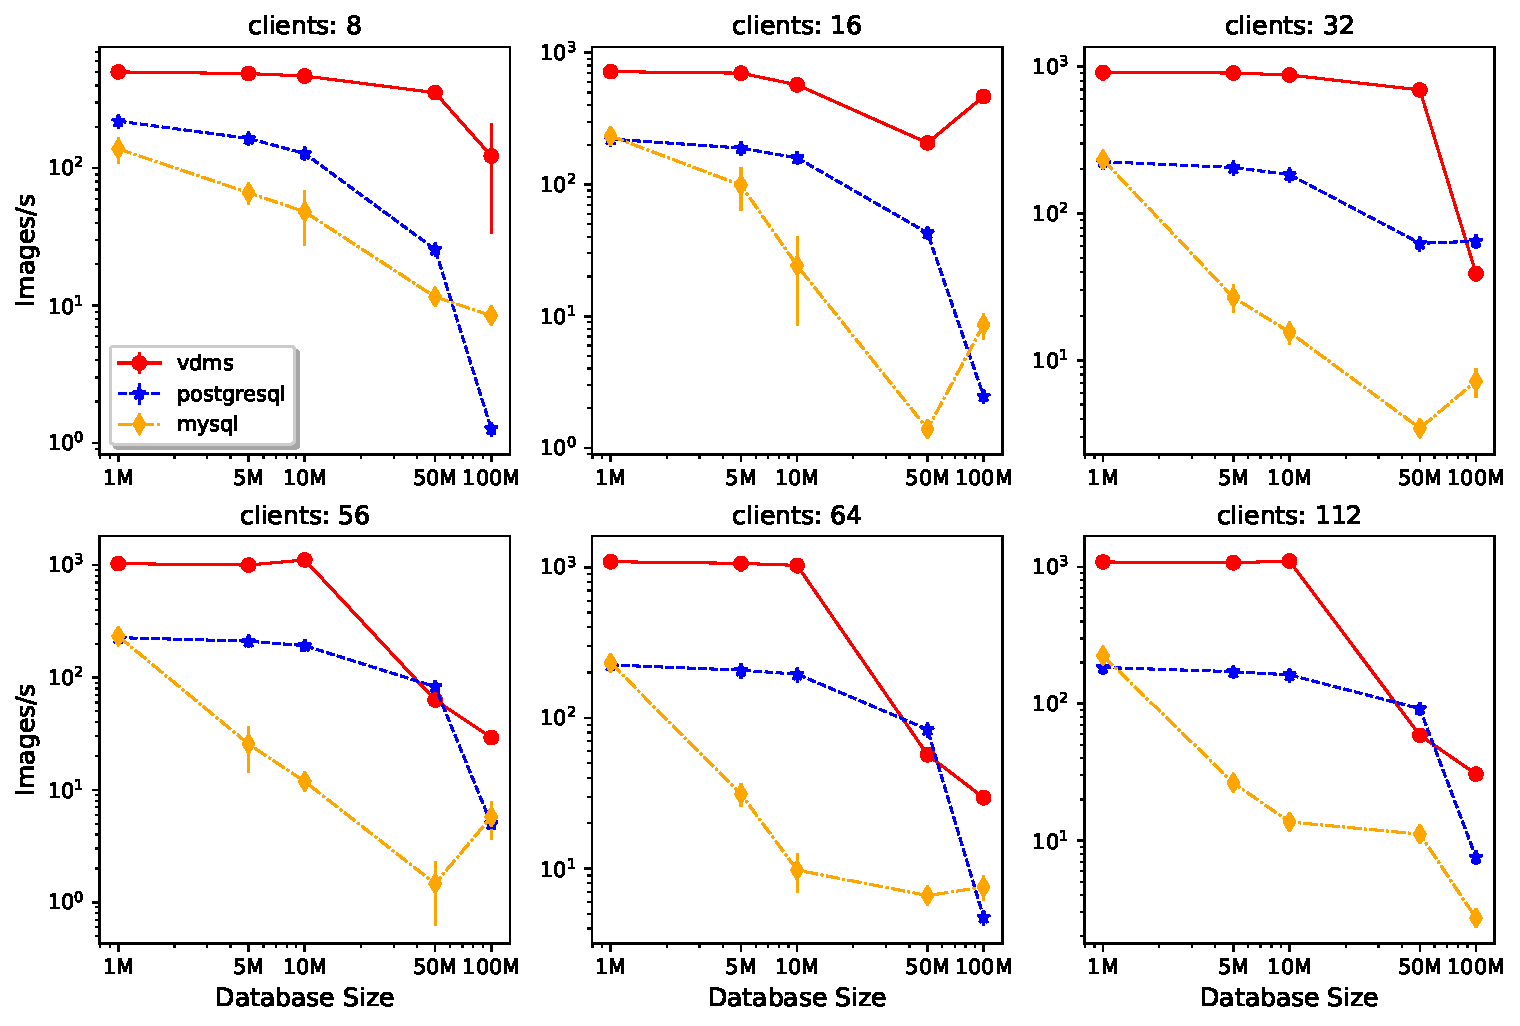
\includegraphics[width=\columnwidth]{figures/plot_q_2tag_resize_or_mosaic_results_throughput_threads}
\caption{Concurrency Analysis on \textit{q4} (\textit{2tag\_or\_resize}) from our use-case
described in the Experimental Setup Section.
We show different number of concurrent clients in different figures for readability reasons.
The experiments show the throughput as images per second for
all systems (VDMS and two baselines) as the database size increases.}
\label{fig:concurrency_comparison_q4}
\end{figure}

In the case of \textit{q4} and \textit{q6}, we see the performance for MySQL
degrades up to 64 concurrent clients, then there's an improvement with 112 concurrent clients.
To further evaluate the concurrency of these queries with an OR operation, we continue by
looking at Figure~\ref{fig:concurrency_comparison_q4}. This figure illustrates a concurrency analysis for
\textit{q4} (\textit{2tag\_resize\_or}) which shows the images per second
delivered by each system as the database size grows (x-axis). We show different number
of concurrent clients in different figures for readability reasons.  For this query,
VDMS delivers higher throughput for databases 1M through 10M for all concurrent clients.
As the number of clients and the size of database grows, the performance for this query
drops and the performance of PostgreSQL becomes more comparable to VDMS. Lets look at the
case with 32 concurrent clients.
In this case, the throughput of VDMS drops drastically with
the 100M database and PostgreSQL outperforms by a small margin.
As the clients increase, we see this trade-off occurs with the 50M database
instead of 100M while in the 100M database, VDMS outperforms both baselines.
In this case, the throughput of PostgreSQL drastically degrades
for the 100M database and the performance of the baseline systems are more comparable.

When considering Figure~\ref{fig:concurrency_comparison_q2}
through Figure~\ref{fig:concurrency_comparison_q4},
there are many reasons why we generally see performance improvement, the main being
that the entire operation (metadata query, image fetching and resizing) happens
on the server side in the case of VDMS, within a single message
exchange between the client and the server.
Many of the inefficiencies that come with combining tools that were designed
for other use cases simply disappear when building a tool that treats
visual entities as first class citizens, as it is the case of VDMS.
Another reason, which is quantifiable in the figures, is that
VDMS sends resized (smaller) versions to the client instead of the full image
to be resized on the client side (as is the case in the baselines).
This is in contrast with the baseline implementations,
where 2 rounds of blocking back-and-forth communication with the server is needed,
as depicted in Figure~\ref{fig:systems}.
Note that one could argue that the opposite will happen
when the resize operation retrieves a an up-sampled (larger) version of the image
instead of a down-sampled (smaller) one.
In practice, retrieving an up-sampled version is not a common use case,
given that up-sampling the image does not add any extra information that can help,
for instance, improve the accuracy of a ML model.
The case of down-sampling the original image is much more common and is the common
practice when it comes to image processing through CNNs \cite{cnn,resnet}.

%% ========= Concurrency Comparison Analysis - END


%% ========= Queries Analysis

\subsubsection{Query Execution Analysis}

\begin{figure}[ht]
% WAS: begin{figure*}[ht]; textwidth
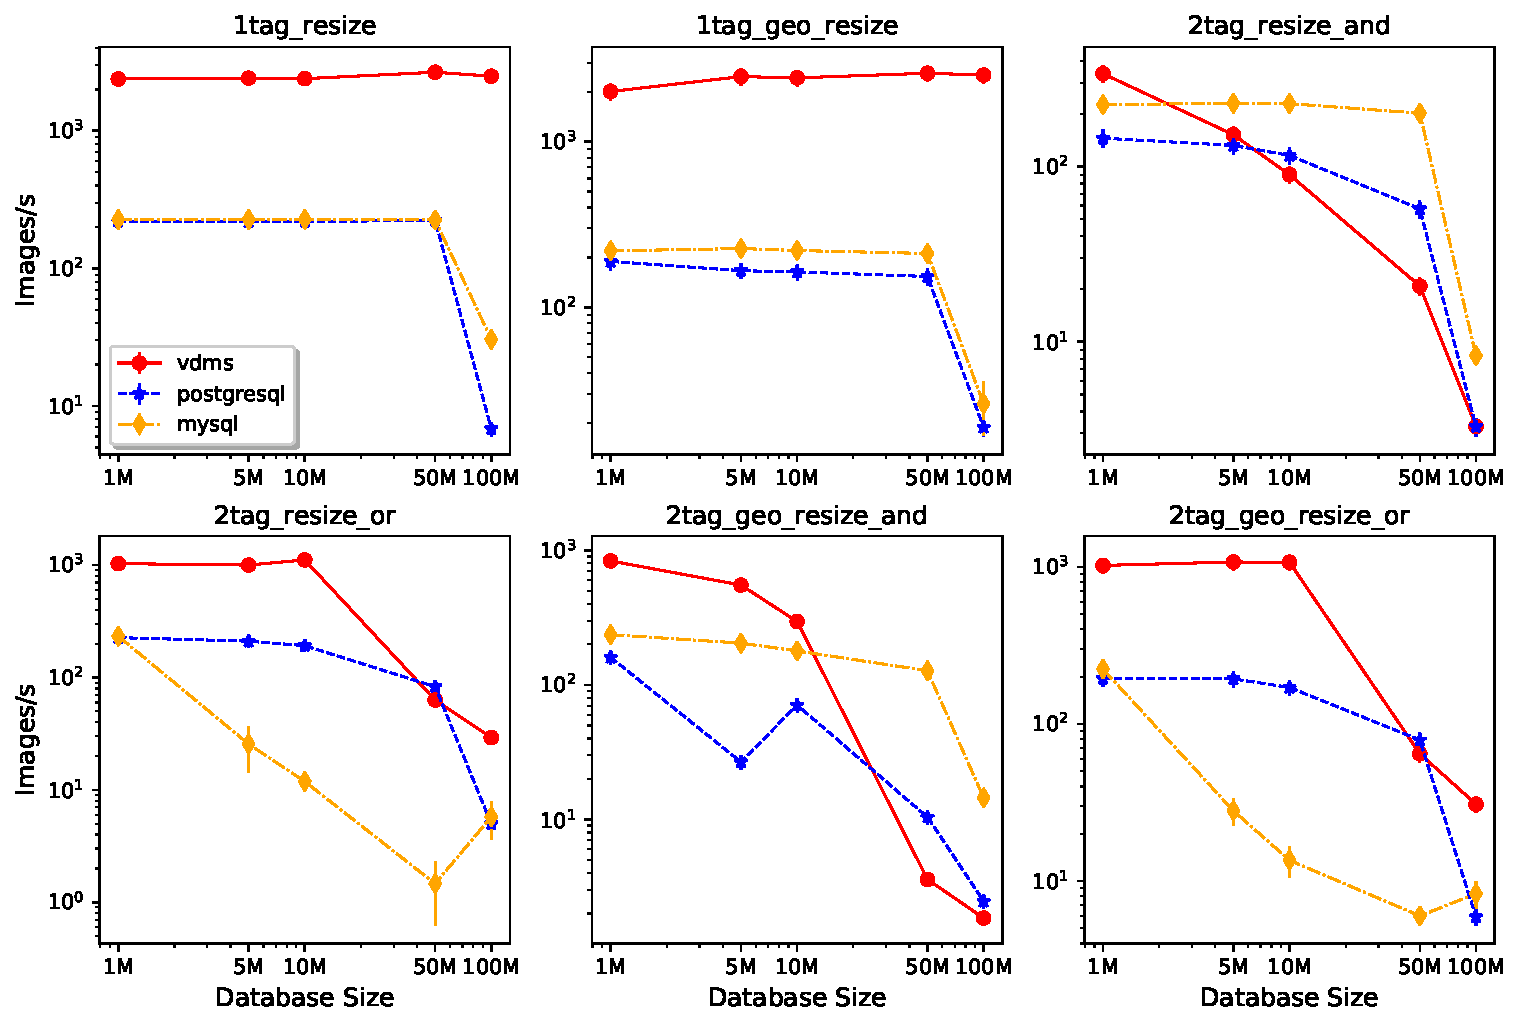
\includegraphics[width=\columnwidth]{figures/plot_th_56_mosaic_results_throughput}
\caption{Throughput Analysis using all queries from our use-case
described in the Experimental Setup Section.
We show queries in different figures for readability reasons.
The experiments show the performance of all systems (VDMS and the two baselines) as the
database size increases.
These queries were run using 56 simultaneous clients (nthr = 56),
and averaged out of 5 runs.}
\label{fig:q_throughput_56}
\end{figure}

The next step in our analysis involved running a set of queries
(described above in this section),
to better understand the performance of the systems under different query conditions.
Figure~\ref{fig:q_throughput_56} shows the evaluation of the
queries we analysed for our use case.
Each figure shows the throughput when retrieving images,
plus operations applied to images when applicable.
The experiments show the performance of all systems (VDMS and two baselines) as the
database size increases in terms of number of images.
These queries were run using 56 simultaneous clients (nthr = 56),
and averaged over 5 runs (niter = 5).
To analyze these plots, one needs to compare the full-line (VDMS) versus the
dotted-lines (two baselines), each plot representing a different query.

For \textit{q1} and \textit{q2}, we can appreciate higher performance being delivered by
VDMS when compared to the baselines, and how this improvement is maintained
as the size of the database increase while
on the other hand, the baseline implementations have a drop in performance
for the 100M database.
For \textit{q3}, we see that VDMS performs best when the database size
is small (1M images), but as the database size increases,
the performance degrades as well.
For this query, MySQL (and in some cases PostgreSQL) outperforms VDMS
for databases larger than 1M.
This also occurs for \textit{q5} but only for databases larger than 10M.
This is entirely attributed to the 2-round process needed for this query,
as we explained before which is more visible in the larger databases.
It is interesting to note that adding filtering by geo-location
(\textit{q5}) decreases the performance as the database sizes scales.
The behaviour is different in the case of \textit{q6},
which also filters by geo-location.
This is attributed to the fact that OR queries involves processing
larger results, and thus does not benefit from the filtering
which is evident when compared to \textit{q4}.

From the first 2 queries, as well as \textit{q4} and
\textit{q6} (with exception to the 50M case),
we clearly see that VDMS outperforms the baseline systems
when retrieving visual data and applying operations.
This is one of the most important finding, as it validates the design principles
of VDMS, which aims to provide scalability and performance acceleration
at the type of queries that require visual data access and transformations.


%% ========= Queries Analysis - END

%% ========= Summary Analysis

\begin{figure*}[ht!]
\centering
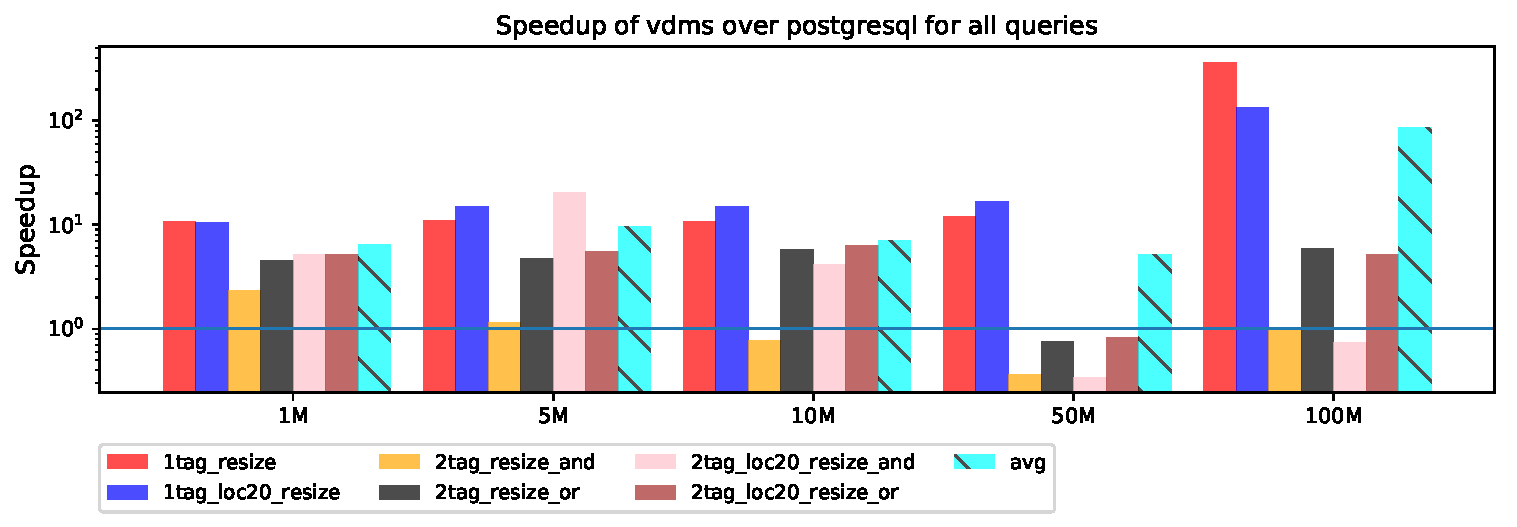
\includegraphics[width=\textwidth]{figures/plot_th_56_query_times_speedup_postgresql}
\caption{Summary of performance gains for all queries.
We see up to 364x speedup (\textit{q1}), and an average of about 85x.
More importantly, we see that the speedup grow as the database size increases,
showing that VDMS scales better than the PostGreSQL baseline.}
\label{fig:summary_postgresql}
\end{figure*}

Finally, Figure~\ref{fig:summary_postgresql} summarizes the results
comparing VDMS and PostgreSQL. A comparison with MySQL is
provided in Figure~\ref{fig:summary_mysql} of the appendix.
In comparison to PostgreSQL, VDMS provides up to 364x speedup
(for the case of \textit{q1}),
and an average improvement in throughput of about 85x. This is
an impressive improvement over the two baseline systems.
More importantly, we see that the speedup increases as the database size grows,
showing that VDMS scales better than the baseline systems.
We also see how \textit{q3} and \textit{q5} have poor performances and scalability
when compared to the baselines as the database size grows.
This evaluation served the
purpose of understanding the importance of VDMS server side operators
that enable more complex queries for our use cases.
The team will address the missing implementation as part of future work.
Most of the performance improvements can be attributed to the design
principles of VDMS, which aims to eliminate the need of combining and
re-purposing systems that were designed to handle types of date other than visual.
VDMS, by design, eliminates all the inefficiencies that result
from a forced integration of components designed for a
different range of applications.

Because of space constraints, we are only showing a subset of our evaluation.

We are making available the all available  of For more details about our comprehensive evaluation.
available
\footnote{https://github.com/luisremis/visual\_storm/tree/master/yfcc100m/python/eval/results}
% TODO. Upload the final version of the plots once we are sure we are not making
% more modifications.

%% ========= Summary Analysis - END

\section{Conclusion}
In this paper, we described VDMS design and implementation and
show a comprehensive evaluation on our Image Search Application.
We use one of the largest publicly available datasets:
The Yahoo Flickr Creative Commons 100M (YFCC100M),
together with the expansions packs that include
machine-generated labels.
We show how VDMS compares against a combination of
industry standard systems, all of which are needed to
replicate only a portion of VDMS' functionality.
We see improvements up to 364x in certain queries,
and an average improvement of about 85x when compared to PostgreSQL+Apache.
When compared to MySQL+Apache, we see up to 96x speedup
and and average improvement of 31x.
The design of VDMS, which was conceived as a
data management system that treats visual entities
as first class citizens, can remove inefficiencies
that result from re-purposing and combining solutions
that were not designed for the job while providing
simpler and richer interfaces.
VDMS' easy-to-use interfaces outperform industry standard systems
with a set of functionalities which, to the best of our knowledge,
are not available in any other single data management solution for visual data.
VDMS was designed for analytics and it can efficiently handle complex queries
which can simplify the design of future applications that rely on visual data.


\section{Acknowledgments}

Not shown during submission.

\begin{comment}
We would like to thank the many people that made this project possible and
helped us through the process, as this work is the results of many efforts.
We want to specially thank our senior technologists Nilesh Jain and 
Ravi Iyer for their full support and input during the duration of the project.
We want to specially acknowledge Philip Lantz and Vishakha Gupta for their help
with PMGD, key to loading large datasets into VDMS.
We want to thank Jim Blakley for his input during the various 
phases of our project, and for advocating and promoting VDMS.
We want to acknowledge the Intel Labs VDMS team for their efforts
open-sourcing and maintaining the system.
We want to thank Jason Gardner for his helping in setting up many of 
the servers and infrastructure needed to conduct our experiments.
\end{comment}



\clearpage

% The following two commands are all you need in the
% initial runs of your .tex file to
% produce the bibliography for the citations in your paper.
\bibliographystyle{plain}
\bibliography{main}
\begin{framed}
\scriptsize

\noindent \textbf{Notices \& Disclaimers}

\noindent Intel technologies may require enabled hardware, software or service activation.

\noindent No product or component can be absolutely secure.

\noindent Your costs and results may vary. 

\noindent \copyright Intel Corporation.  Intel, the Intel logo, and other Intel marks are trademarks of Intel Corporation or its subsidiaries.  Other names and brands may be claimed as the property of others. 

\noindent Intel does not control or audit third-party data.  You should consult other sources to evaluate accuracy.

\noindent Intel disclaims all express and implied warranties, including without limitation, the implied warranties of merchantability, fitness for a particular purpose, and non-infringement, as well as any warranty arising from course of performance, course of dealing, or usage in trade.

% \copyright  Intel Corporation.  Intel, the Intel logo, and other Intel marks are trademarks of Intel Corporation or its subsidiaries.  Other names and brands may be claimed as the property of others.

% Performance results are based on testing as of dates shown in configurations and may not reflect all publicly available security updates.  See backup for configuration details.  No product or component can be absolutely secure.

% Your costs and results may vary.

% Intel technologies may require enabled hardware, software or service activation.

% Software and workloads used in performance tests may have been optimized for performance only on Intel microprocessors.  Performance tests, such as SYSmark and MobileMark, are measured using specific computer systems, components, software, operations and functions.  Any change to any of those factors may cause the results to vary.  You should consult other information and performance tests to assist you in fully evaluating your contemplated purchases, including the performance of that product when combined with other products.   For more complete information visit www.intel.com/benchmarks.

% Intel's compilers may or may not optimize to the same degree for non-Intel microprocessors for optimizations that are not unique to Intel microprocessors. These optimizations include SSE2, SSE3, and SSSE3 instruction sets and other optimizations. Intel does not guarantee the availability, functionality, or effectiveness of any optimization on microprocessors not manufactured by Intel. Microprocessor-dependent optimizations in this product are intended for use with Intel microprocessors. Certain optimizations not specific to Intel microarchitecture are reserved for Intel microprocessors. Please refer to the applicable product User and Reference Guides for more information regarding the specific instruction sets covered by this notice.  Notice Revision \#20110804
\end{framed}


\clearpage
\appendix

\section{APPENDIX - Video Evaluation}
%=========================================
\subsection{Video Search}
\label{videos}

VDMS provides full support for video storage and operations,
in a similar way it does for images.
This includes support for encoding, decoding, and transcoding of
\textit{mp4}, \textit{avi}, and \textit{mov} containers,
as well as support for \textit{xvid}, \textit{H.263} and \textit{H.264} encoders.
This is supported through the Visual Compute Module that provides an abstraction
layer on top of OpenCV~\cite{opencv} and \textit{libffmpeg}\cite{ffmpeg}.
All operations supported for images in VDMS are also supported at the
video and frame level of the API.
On top of that, there are a number of video-specific operations that
are supported, such as the interval operations,
enabling users to retrieve clips at different
frames-per-second (FPS) versions of the video.

We evaluate the performance and scalability of the video management
capabilities offered by VDMS.
Handling video in a general way is a complex task.
Some of this complexity comes from the existence of a variety of open and
proprietary implementations, different encoding techniques and container
formats, and different parameters of the video itself that are
application-dependent, like frames per second, lossy compression, etc.
When it comes to video, ad-hoc solutions have a large number of parameters that
can be tuned.
Together with that, there is no system that enables transactional
operations over videos files in the way VDMS does.
Because of this, we focus our efforts on understanding variations in the
performance of VDMS and its scalability, rather than comparing
it to a baseline that would not represent a fair
comparison for either of the systems.

\begin{figure*}[ht!]
\centering
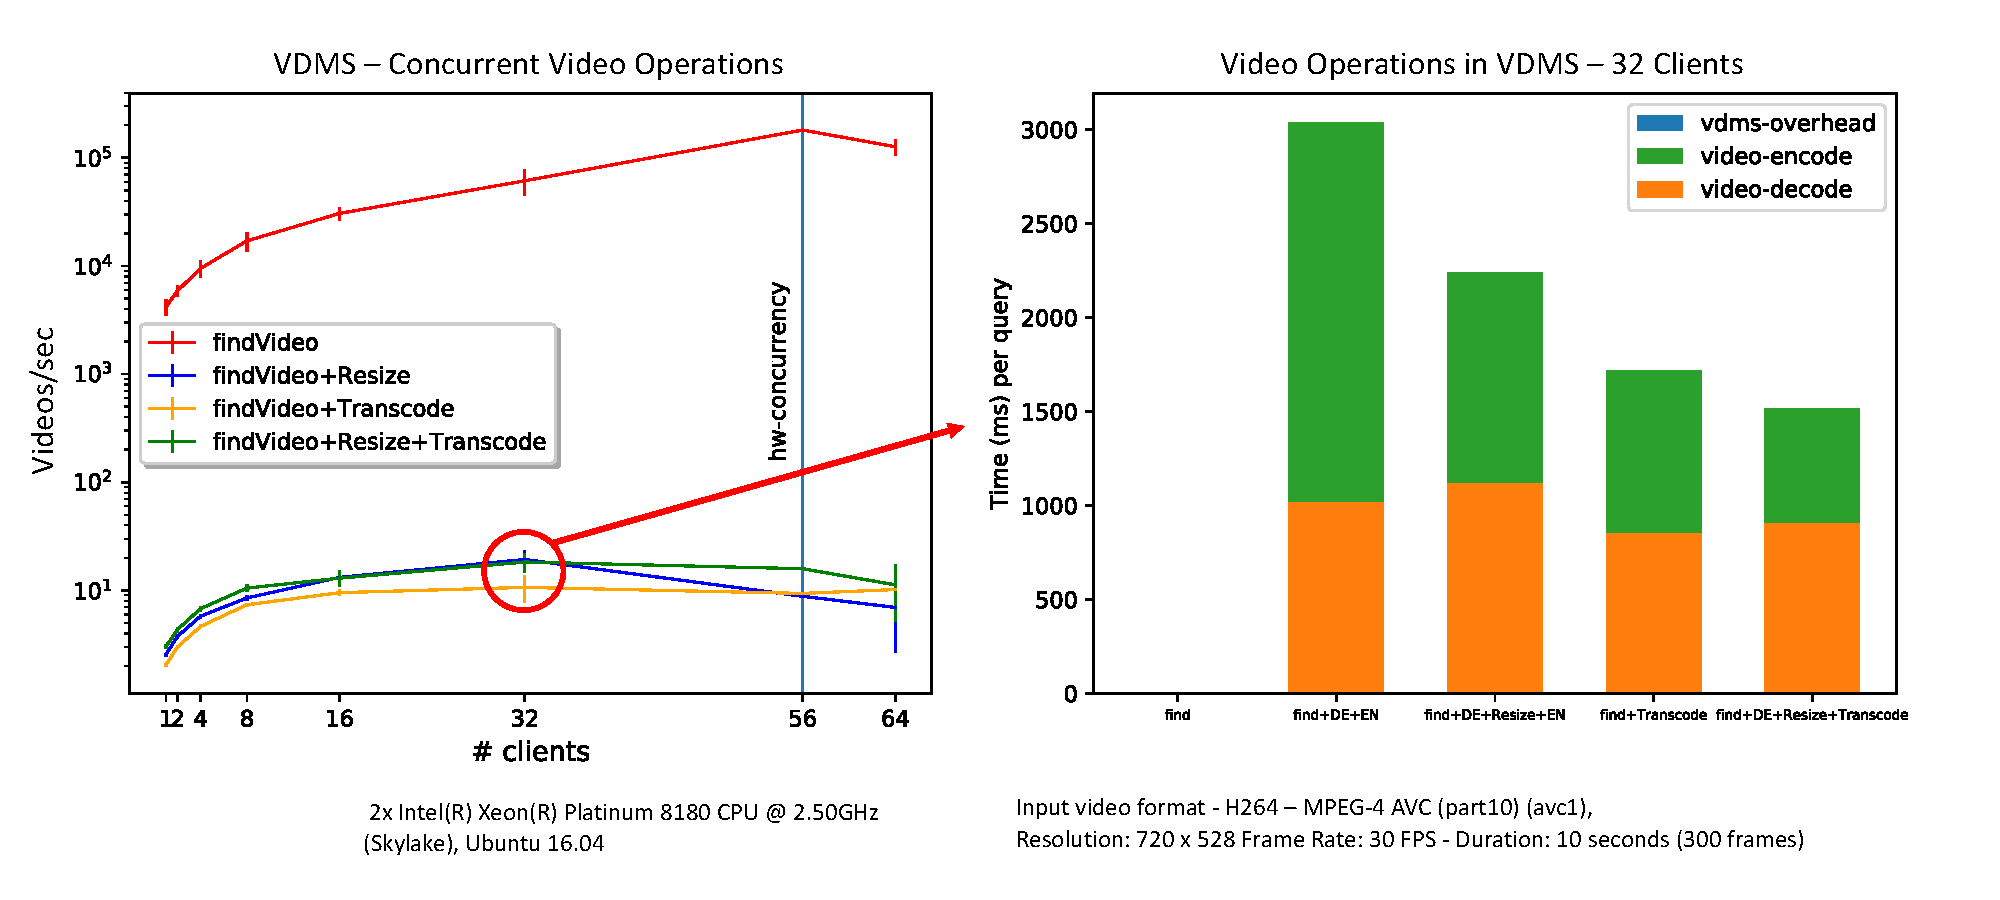
\includegraphics[width=\textwidth]{figures/video_overhead}
\caption{Analysis of video operations. The left figure shows the video throughput (videos per sec) as the number of concurrent clients increase and the right figure breaks down the different components of the
queries using 32 clients.}
\label{fig:video}
\end{figure*}

All this functionality is provided and integrated with the rest of the
metadata API as part of the comprehensive VDMS interface.
This makes it possible for users to interact with metadata and video in
a transactional manner, enabling users to run queries like:
"Retrieve all the videos where there is a \textit{lake} with
probability higher than 0.86, converting all videos to \textit{H.264}
\textit{mp4} of size 224x224".
Appendix shows a sample of how this query would be implemented using the VDMS API
\footnote{https://github.com/IntelLabs/vdms/wiki/FindVideo}.
In particular, this functionality was used internally to select a subset
of videos with the right licenses for a video summarization application.

To the best of our knowledge, there is no solution that can provide
all the functionality mentioned above, behind a single interface
that also allows users to interact with images and metadata.
Implementing a baseline, like we did for images, is significantly more complex
due to the parametrization of video encodings and containers,
as explained at the beginning of this section.
For this reason, we chose to make a study using VDMS in various scenarios,
and analysis of scalability and the impact of having the overhead of VDMS' Request
Server in the overall access time and throughput.

Figure~\ref{fig:video} shows the analysis of different queries aimed
at retrieving a video using the VDMS interface.
We show how VDMS throughput increases when serving
a video object as the number of simultaneous clients increases, as well as the
overhead operations introduced in the overall query execution time.
The figure on the left compares the number of video transaction per second
(i.e., number of videos returned per second) when different operations
are executed as part of the transaction. The upper-bound of this would be
simply returning the video as-is (without running any encoding/decoding or
operation), represented by the red line. This query is the upper-limit because
it essentially translates to reading the video from the file-system and sending
it over a TCP/IP socket, without any other overhead or operations.

\begin{listing}[ht!]
\begin{minted}[frame=single,
               framesep=3mm,
               linenos=true,
               xleftmargin=21pt,
               tabsize=4]{js}
"FindEntity"{
    "class": "autotag",
    "constraints": {
        "name": ["==", "lake"]
    }
    "_ref" : 1
},
"FindVideo":{
    "container": "mp4",
    "codec": "h.264",
    "link": {
        "ref":1,
        "constraints": {
            "prob": [">=", 0.86]
        }
    }
    "operations": [{
        "type": "resize",
        "height": 1080,
        "width":  1920,
    }]
}

\end{minted}
\caption{Sample Query for Video -
The query expresses the following:
Find all videos connected to the autotag \textit{lake}
with probability higher than 0.86, apply a resize operation
to make the video 1920×1080, and convert to "mp4" file,
using H.264 encoding.}
\label{findvideo}
\end{listing}

We also run a set of other queries that involve, showed in Figure~\ref{fig:video}:
(a) running a resize operation on the video and, consequently,
decoding and encoding operations as well (blue line),
(b) transcoding, meaning the use of a different container and encoder
than the one originally used (yellow line), and
(c) both resize and transcoding.
Note that the resize operation (blue and green lines) performs a downsize,
which translates in less data being sent over the wire.
This is specially noticeable when supporting 32 simultaneous clients,
where the system provides more videos per second due to sending less data to
the client, when compared to just transcoding and not resizing (yellow line).
We can see that the system performs best when using all the physical cores,
and this can be attributed to the compute-bound nature of video
encoding, decoding, and processing.

It is important to note an almost 3 orders of magnitude drop in performance
when including operations as part of the query.
We wanted to understand where most of the time was spent on the queries,
and optimize the Request Server and Visual Compute Module
if necessary. For this, we run the experiment shown at
Figure~\ref{fig:video} (right) which breaks down the different components of the
queries. This figure shows that more than 97\% of the query execution is spent
on encoding/decoding operations, which is well-known to be a
compute intensive operation\cite{videosgoogle}.
On the one hand, this result shows that VDMS barely introduces any overhead.
On the other hand, this result means a limit on the opportunities
for optimization for video queries given that biggest time factors
are accounted by encoding/decoding, which is outside the scope of VDMS.
This result was the call to action for one optimization we will include
in future releases of VDMS, which involves using \textit{ffmpeg} C++ API to
limit the number of frames being encoded/decoded when possible.
This functionality will prevent encoding/decoding to happen on all frames
when users only need to retrieve a subset of the frames in the video.

%=========================================

\clearpage

\section{APPENDIX - Similarity Search Evaluation}

\begin{figure*}[ht!]
\centering
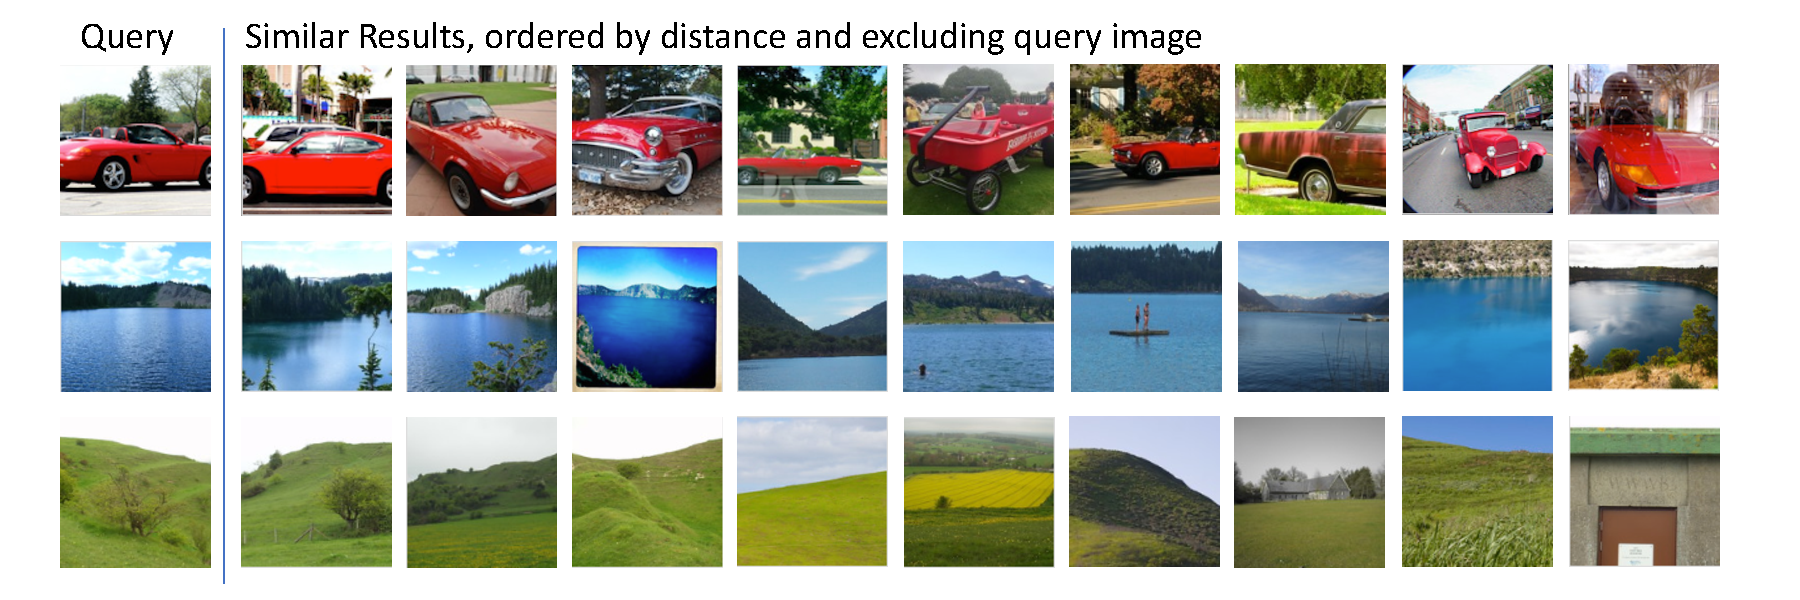
\includegraphics[width=\textwidth]{figures/feature_img_results}
\caption{Sample Results of Similarity Search}
\label{fig:similarity}
\end{figure*}

\subsection{Similarity Search}
\label{features}

Another key differentiating factor of VDMS is that it allows the creation of
indexes for high-dimensional feature vectors and the insertion of
these feature vectors associated with entities, images, and/or videos.
Feature vectors are intermediate results of various machine
learning or computer vision algorithms when run on visual data.
Feature vectors are also known as \textit{descriptors}
or \textit{visual descriptors}. We use these terms interchangeably.
These descriptors can be classified, labeled, and used to build search
indexes. There are many in-memory libraries that are designed for
this task~\cite{flann, faiss}.

% We analyze the behavior of the feature vector functionality in VDMS,
% and an evaluation of the different trade-offs that the systems offers for
% application developers. For this, we implemented an image-search application
% based on \textit{similarity} search.

Using the VDMS API, users can manage feature vector indexes,
query previously inserted elements,
run a k-nearest neighbor search (\textit{knn}), and express relationships
between existing images or descriptors and
the newly inserted descriptors.
By natively supporting descriptors and \textit{knn},
VDMS allows out-of-the-box classification functionalities for many applications
\footnote{https://github.com/\{Not shown during submission\}}.
% \footnote{https://github.com/IntelLabs/vdms/wiki/ClassifyDescriptor}.

For this work, and as part of a comprehensive image search implementation,
we have used 4096-dimensional descriptors extracted from every image
(and first frame of every video) from the YFCC100M dataset
and created a collection of these feature vectors in VDMS to
perform similarity search (i.e., find images that are
\textit{similar} to an query (input) image).
\textit{Similarity} in this particular case is defined as closeness
in a 4096-dimensional space using euclidean distance as the metric.

The process of loading descriptors in VDMS is simple.
First, the user has to create a DescriptorSet, using a single command.
At creation of the DescriptorSet, the dimensionality of the descriptors
is specified, together with the desired indexing method and the desired metric
for computing distances (Euclidean Distance, \textit{L2},
or Inner Product, \textit{IP}).
Once the DescriptorSet is created, descriptors can be inserted to the set.
After the descriptors are inserted, a similarity search can be performed.

Figure~\ref{fig:similarity} shows 3 examples of a query image (on the left),
and images returned as \textit{similar} by VDMS.
The input is a descriptor generated after a query image.
The \textit{query input} descriptor is sent to VDMS as part of the query,
VDMS uses that descriptor to find similar ones,
and retrieves the images associated with those \textit{similar} descriptors.
We show this as an example of the functionality and to depict
how the feature vectors provided by the dataset can be used,
but we also provide an analytical approach to
the trade-off between accuracy and execution time in our system.
It is important to note that the accuracy of the results is entirely tied
to the quality of the descriptors chosen by the applications.
The quality of the similarity result will be tied to the quality
of the descriptor extraction that the application is using.

\begin{figure*}[ht]
\centering
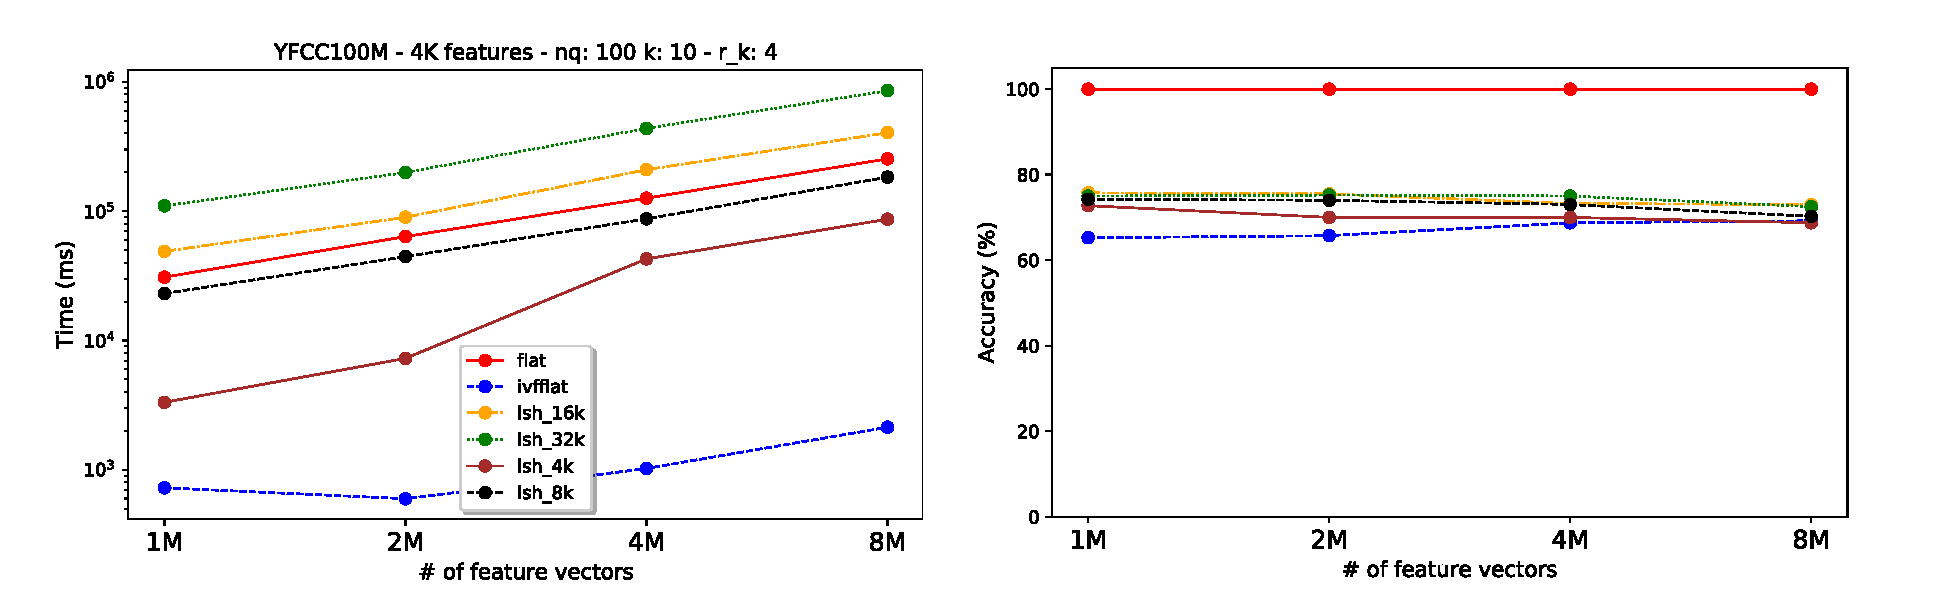
\includegraphics[width=\textwidth]{figures/features_alternatives}
\caption{Feature Vector Evaluation: Trade-off between query execution speed
and accuracy of the results, using ground-truth data for computing accuracy.
For this evaluation, we query the 10 closest neighbors (k = 10), and compute
accuracy using recall at 4 (r\_k = 4) (i.e. percentage of the top 4 ground-truth
results that is present within the top 10 computed neighbors).
We average the query execution time and accuracy for 100 queries (nq = 100).}
\label{fig:features_eval}
\end{figure*}

\begin{figure*}[ht]
\centering
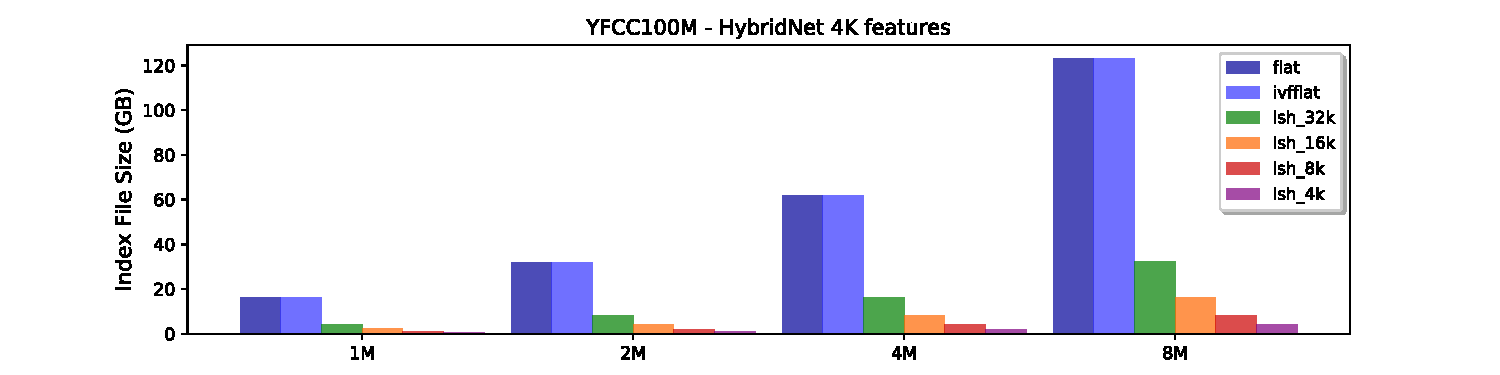
\includegraphics[width=\textwidth]{figures/features_disksize}
\caption{Feature Collection Size in Disk}
\label{fig:features_size_does_matter}
\end{figure*}

As mentioned before, VDMS provides different levels of customization of the
indexes created for a descriptor set, that includes the indexing techniques
and the metric for similarity.
These different indexing techniques come with different trade-offs in terms
of speed of search and accuracy of the computation.
VDMS aims to provide functionality that is agnostics to application-specific
techniques, enabling features that are generic to visual data processing
applications.
Figure~\ref{fig:features_eval} shows an analysis at the different indexing
techniques provided by VDMS and its trades-off between accuracy and query
execution speed, for a single threaded client.
For this evaluation, we query the 10 closest neighbors (k = 10), and compute
accuracy using recall at 4 (r\_k = 4) (i.e. percentage of the top 4 ground-truth
results that is present within the top 10 computed neighbors).
We average the query execution time and accuracy for 100 queries (nq = 100).
The \textit{flat} index (red line) implements exact search and
represents ground-truth, which explain why the
accuracy is always 100\% in the plot on the right.
The other indexes implement \textit{approximate search},
which trades-off between accuracy and speed of search~\cite{flann, faiss}.
We have also tried the \textit{ivfflat} index (inverted file index), as well as
\textit{LSH}-based indexes using a different number of bits per descriptor
\footnote{https://github.com/facebookresearch/faiss/wiki/Faiss-indexes}.
Results show how \textit{ivfflat} is the fastest option but it comes with a trade-off
of about 30\% loss in accuracy, while simple brute-force search
is among the slowest options at the expenses of 100\% accuracy,
meaning exact search.

Another important trade-off to be made is with respect to space efficiency:
The DescriptorSet can grow very large and expensive to load and manage.
In this particular case, 4096-dimensional descriptors for 100M elements
translates into 1TB of data, only in raw floating-point data alone
(without accounting for any metadata or indexes associated with it).
This component is very important for the overall analysis on which
index structure to use because a large set of descriptors may not fit in memory
and thus cause a pressure on the IO system while retrieving descriptors
for computing distance.
This can severely impact the overall query execution time.
When the DescriptorSet grows significantly large,
it may be worth trading off accuracy for speed and space.
Figure~\ref{fig:features_size_does_matter} shows the different indexes and
their size in disk. These indexes already contain all the descriptors (or
a quantized version of them in the case of LSH~\cite{lsh}),
and can be loaded in memory directly when it fits.
Note how, because of quantization of the descriptors, \textit{LSH} provides a
significantly lower space foot print, which can be a great option for
large collections of descriptors when accuracy is not a main factor.
It is not uncommon to sacrifice accuracy as images and videos are captured
using a noise sensor (i.e., the camera), and an approximate search
in many cases can provide the necessary accuracy for applications
to achieve their goals.


% \section{APPENDIX - API Samples}

% \begin{appendix}

% \begin{listing}[ht!]
% \begin{minted}[frame=single,
%               framesep=3mm,
%               linenos=true,
%               xleftmargin=21pt,
%               tabsize=4]{js}
% "FindEntity"{     
%     "class": "autotag",
%     "constraints": { 
%         "name": ["==", "alligator"]
%     }
%     "_ref" : 1
% },
% "FindImage":{
%     "format": "png",
%     "link": {
%         "ref":1,
%         "constraints": {
%             "prob": [">=", 0.66]
%         }
%     }
%     "operations": [{
%         "type": "resize",
%         "height": 224,
%         "width":  224,
%     }]
% }

% \end{minted}
% \caption{Sample Query for Images - 
% The query expresses the following: 
% Find all the images connected to the autotag \textit{alligator} 
% with probability higher than 0.66, apply a resize operation
% to make the images 224x224, and convert to "png".} 
% \label{findimage}
% \end{listing}

% \begin{listing}[t!]
% \begin{minted}[frame=single,
%               framesep=3mm,
%               linenos=true,
%               xleftmargin=21pt,
%               tabsize=4]{js}
% "FindEntity"{     
%     "class": "autotag",
%     "constraints": { 
%         "name": ["==", "alligator"]
%     }
%     "_ref" : 1
% },
% "FindImage":{
%     "format": "png",
%     "link": {
%         "ref":1,
%         "constraints": {
%             "prob": [">=", 0.66]
%         }
%     }, 
%     "constraints": {
%         "latitude": [">=", 36.23433, 
%                      "<=", 38.23433]
%         "longitude":[">=", -114.80666, 
%                      "<=", -116.80666]
%     },
%     "operations": [{
%         "type": "resize",
%         "height": 224,
%         "width":  224,
%     }, {
%         "type": "rotate",
%         "angle": 45.34
%     }]
% }

% \end{minted}
% \caption{Sample Query for Images - 
% The query expresses the following: 
% Find all the images connected to the autotag \textit{alligator} 
% with probability higher than 0.66, 
% filter by latitude and longitude within 1 degree, 
% apply a resize operation to make the images 224x224
% and rotate the image 45.34 degrees, 
% and return the images as "png" files.} 
% \label{findimagegeo}
% \end{listing}

% \end{appendix}

\appendix

\section{APPENDIX - Video Evaluation}
%=========================================
\subsection{Video Search}
\label{videos}

VDMS provides full support for video storage and operations,
in a similar way it does for images.
This includes support for encoding, decoding, and transcoding of
\textit{mp4}, \textit{avi}, and \textit{mov} containers,
as well as support for \textit{xvid}, \textit{H.263} and \textit{H.264} encoders.
This is supported through the Visual Compute Module that provides an abstraction
layer on top of OpenCV~\cite{opencv} and \textit{libffmpeg}\cite{ffmpeg}.
All operations supported for images in VDMS are also supported at the
video and frame level of the API.
On top of that, there are a number of video-specific operations that
are supported, such as the interval operations,
enabling users to retrieve clips at different
frames-per-second (FPS) versions of the video.

We evaluate the performance and scalability of the video management
capabilities offered by VDMS.
Handling video in a general way is a complex task.
Some of this complexity comes from the existence of a variety of open and
proprietary implementations, different encoding techniques and container
formats, and different parameters of the video itself that are
application-dependent, like frames per second, lossy compression, etc.
When it comes to video, ad-hoc solutions have a large number of parameters that
can be tuned.
Together with that, there is no system that enables transactional
operations over videos files in the way VDMS does.
Because of this, we focus our efforts on understanding variations in the
performance of VDMS and its scalability, rather than comparing
it to a baseline that would not represent a fair
comparison for either of the systems.

\begin{figure*}[ht!]
\centering
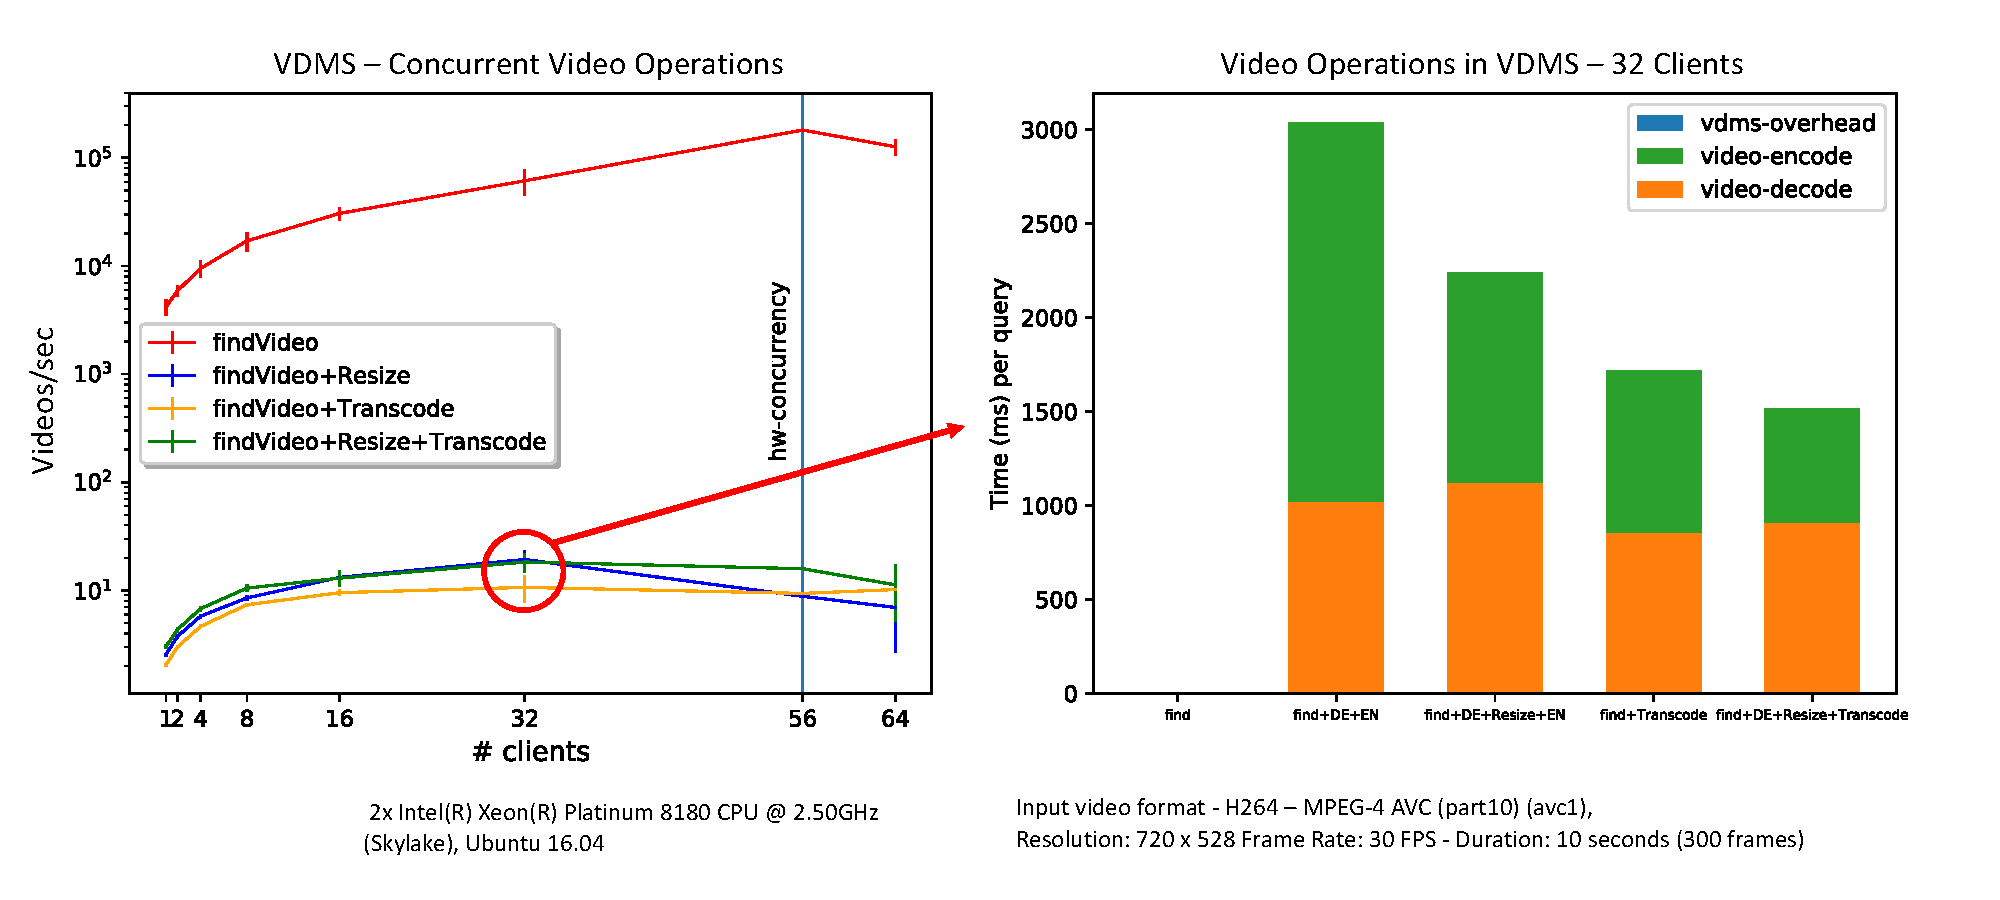
\includegraphics[width=\textwidth]{figures/video_overhead}
\caption{Analysis of video operations. The left figure shows the video throughput (videos per sec) as the number of concurrent clients increase and the right figure breaks down the different components of the
queries using 32 clients.}
\label{fig:video}
\end{figure*}

All this functionality is provided and integrated with the rest of the
metadata API as part of the comprehensive VDMS interface.
This makes it possible for users to interact with metadata and video in
a transactional manner, enabling users to run queries like:
"Retrieve all the videos where there is a \textit{lake} with
probability higher than 0.86, converting all videos to \textit{H.264}
\textit{mp4} of size 224x224".
Appendix shows a sample of how this query would be implemented using the VDMS API
\footnote{https://github.com/IntelLabs/vdms/wiki/FindVideo}.
In particular, this functionality was used internally to select a subset
of videos with the right licenses for a video summarization application.

To the best of our knowledge, there is no solution that can provide
all the functionality mentioned above, behind a single interface
that also allows users to interact with images and metadata.
Implementing a baseline, like we did for images, is significantly more complex
due to the parametrization of video encodings and containers,
as explained at the beginning of this section.
For this reason, we chose to make a study using VDMS in various scenarios,
and analysis of scalability and the impact of having the overhead of VDMS' Request
Server in the overall access time and throughput.

Figure~\ref{fig:video} shows the analysis of different queries aimed
at retrieving a video using the VDMS interface.
We show how VDMS throughput increases when serving
a video object as the number of simultaneous clients increases, as well as the
overhead operations introduced in the overall query execution time.
The figure on the left compares the number of video transaction per second
(i.e., number of videos returned per second) when different operations
are executed as part of the transaction. The upper-bound of this would be
simply returning the video as-is (without running any encoding/decoding or
operation), represented by the red line. This query is the upper-limit because
it essentially translates to reading the video from the file-system and sending
it over a TCP/IP socket, without any other overhead or operations.

\begin{listing}[ht!]
\begin{minted}[frame=single,
               framesep=3mm,
               linenos=true,
               xleftmargin=21pt,
               tabsize=4]{js}
"FindEntity"{
    "class": "autotag",
    "constraints": {
        "name": ["==", "lake"]
    }
    "_ref" : 1
},
"FindVideo":{
    "container": "mp4",
    "codec": "h.264",
    "link": {
        "ref":1,
        "constraints": {
            "prob": [">=", 0.86]
        }
    }
    "operations": [{
        "type": "resize",
        "height": 1080,
        "width":  1920,
    }]
}

\end{minted}
\caption{Sample Query for Video -
The query expresses the following:
Find all videos connected to the autotag \textit{lake}
with probability higher than 0.86, apply a resize operation
to make the video 1920×1080, and convert to "mp4" file,
using H.264 encoding.}
\label{findvideo}
\end{listing}

We also run a set of other queries that involve, showed in Figure~\ref{fig:video}:
(a) running a resize operation on the video and, consequently,
decoding and encoding operations as well (blue line),
(b) transcoding, meaning the use of a different container and encoder
than the one originally used (yellow line), and
(c) both resize and transcoding.
Note that the resize operation (blue and green lines) performs a downsize,
which translates in less data being sent over the wire.
This is specially noticeable when supporting 32 simultaneous clients,
where the system provides more videos per second due to sending less data to
the client, when compared to just transcoding and not resizing (yellow line).
We can see that the system performs best when using all the physical cores,
and this can be attributed to the compute-bound nature of video
encoding, decoding, and processing.

It is important to note an almost 3 orders of magnitude drop in performance
when including operations as part of the query.
We wanted to understand where most of the time was spent on the queries,
and optimize the Request Server and Visual Compute Module
if necessary. For this, we run the experiment shown at
Figure~\ref{fig:video} (right) which breaks down the different components of the
queries. This figure shows that more than 97\% of the query execution is spent
on encoding/decoding operations, which is well-known to be a
compute intensive operation\cite{videosgoogle}.
On the one hand, this result shows that VDMS barely introduces any overhead.
On the other hand, this result means a limit on the opportunities
for optimization for video queries given that biggest time factors
are accounted by encoding/decoding, which is outside the scope of VDMS.
This result was the call to action for one optimization we will include
in future releases of VDMS, which involves using \textit{ffmpeg} C++ API to
limit the number of frames being encoded/decoded when possible.
This functionality will prevent encoding/decoding to happen on all frames
when users only need to retrieve a subset of the frames in the video.

%=========================================

\clearpage

\section{APPENDIX - Similarity Search Evaluation}

\begin{figure*}[ht!]
\centering
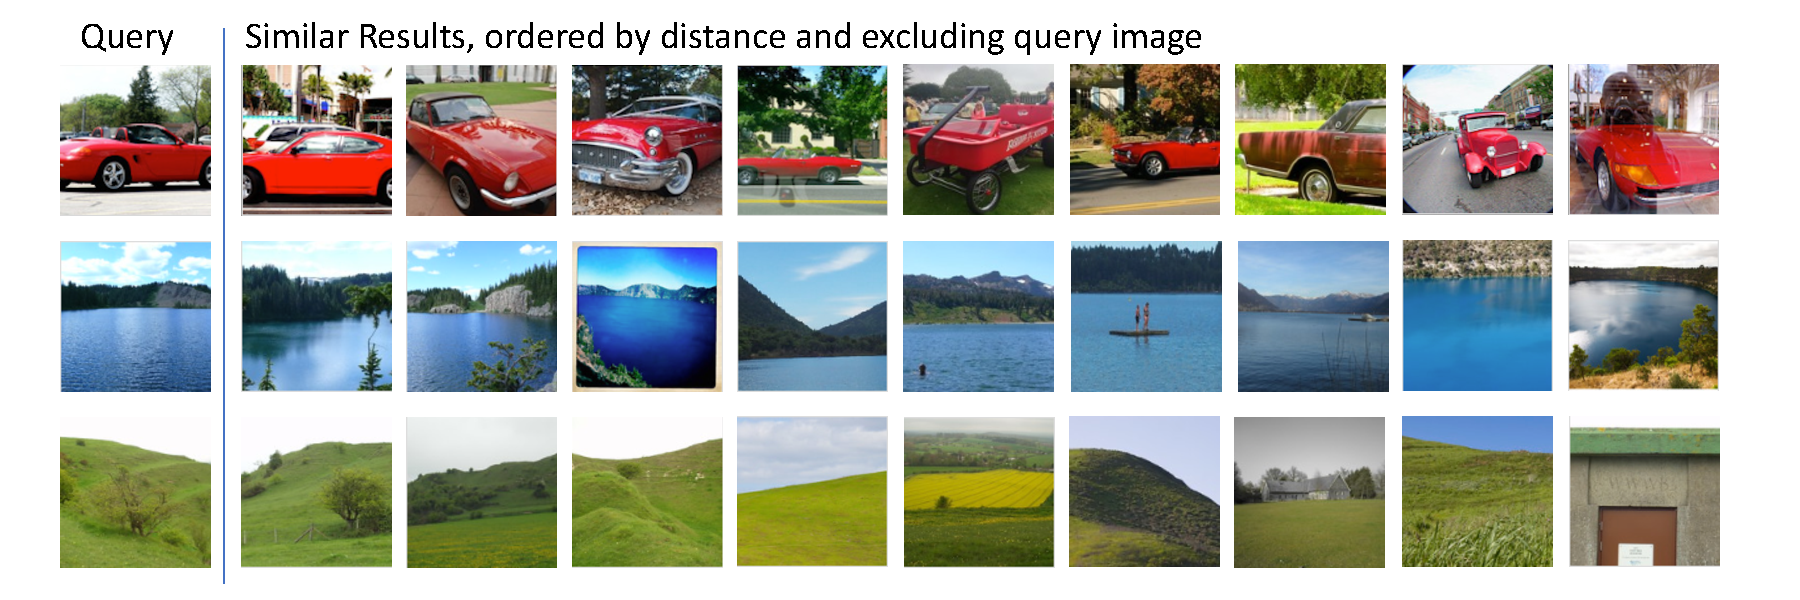
\includegraphics[width=\textwidth]{figures/feature_img_results}
\caption{Sample Results of Similarity Search}
\label{fig:similarity}
\end{figure*}

\subsection{Similarity Search}
\label{features}

Another key differentiating factor of VDMS is that it allows the creation of
indexes for high-dimensional feature vectors and the insertion of
these feature vectors associated with entities, images, and/or videos.
Feature vectors are intermediate results of various machine
learning or computer vision algorithms when run on visual data.
Feature vectors are also known as \textit{descriptors}
or \textit{visual descriptors}. We use these terms interchangeably.
These descriptors can be classified, labeled, and used to build search
indexes. There are many in-memory libraries that are designed for
this task~\cite{flann, faiss}.

% We analyze the behavior of the feature vector functionality in VDMS,
% and an evaluation of the different trade-offs that the systems offers for
% application developers. For this, we implemented an image-search application
% based on \textit{similarity} search.

Using the VDMS API, users can manage feature vector indexes,
query previously inserted elements,
run a k-nearest neighbor search (\textit{knn}), and express relationships
between existing images or descriptors and
the newly inserted descriptors.
By natively supporting descriptors and \textit{knn},
VDMS allows out-of-the-box classification functionalities for many applications
\footnote{https://github.com/\{Not shown during submission\}}.
% \footnote{https://github.com/IntelLabs/vdms/wiki/ClassifyDescriptor}.

For this work, and as part of a comprehensive image search implementation,
we have used 4096-dimensional descriptors extracted from every image
(and first frame of every video) from the YFCC100M dataset
and created a collection of these feature vectors in VDMS to
perform similarity search (i.e., find images that are
\textit{similar} to an query (input) image).
\textit{Similarity} in this particular case is defined as closeness
in a 4096-dimensional space using euclidean distance as the metric.

The process of loading descriptors in VDMS is simple.
First, the user has to create a DescriptorSet, using a single command.
At creation of the DescriptorSet, the dimensionality of the descriptors
is specified, together with the desired indexing method and the desired metric
for computing distances (Euclidean Distance, \textit{L2},
or Inner Product, \textit{IP}).
Once the DescriptorSet is created, descriptors can be inserted to the set.
After the descriptors are inserted, a similarity search can be performed.

Figure~\ref{fig:similarity} shows 3 examples of a query image (on the left),
and images returned as \textit{similar} by VDMS.
The input is a descriptor generated after a query image.
The \textit{query input} descriptor is sent to VDMS as part of the query,
VDMS uses that descriptor to find similar ones,
and retrieves the images associated with those \textit{similar} descriptors.
We show this as an example of the functionality and to depict
how the feature vectors provided by the dataset can be used,
but we also provide an analytical approach to
the trade-off between accuracy and execution time in our system.
It is important to note that the accuracy of the results is entirely tied
to the quality of the descriptors chosen by the applications.
The quality of the similarity result will be tied to the quality
of the descriptor extraction that the application is using.

\begin{figure*}[ht]
\centering
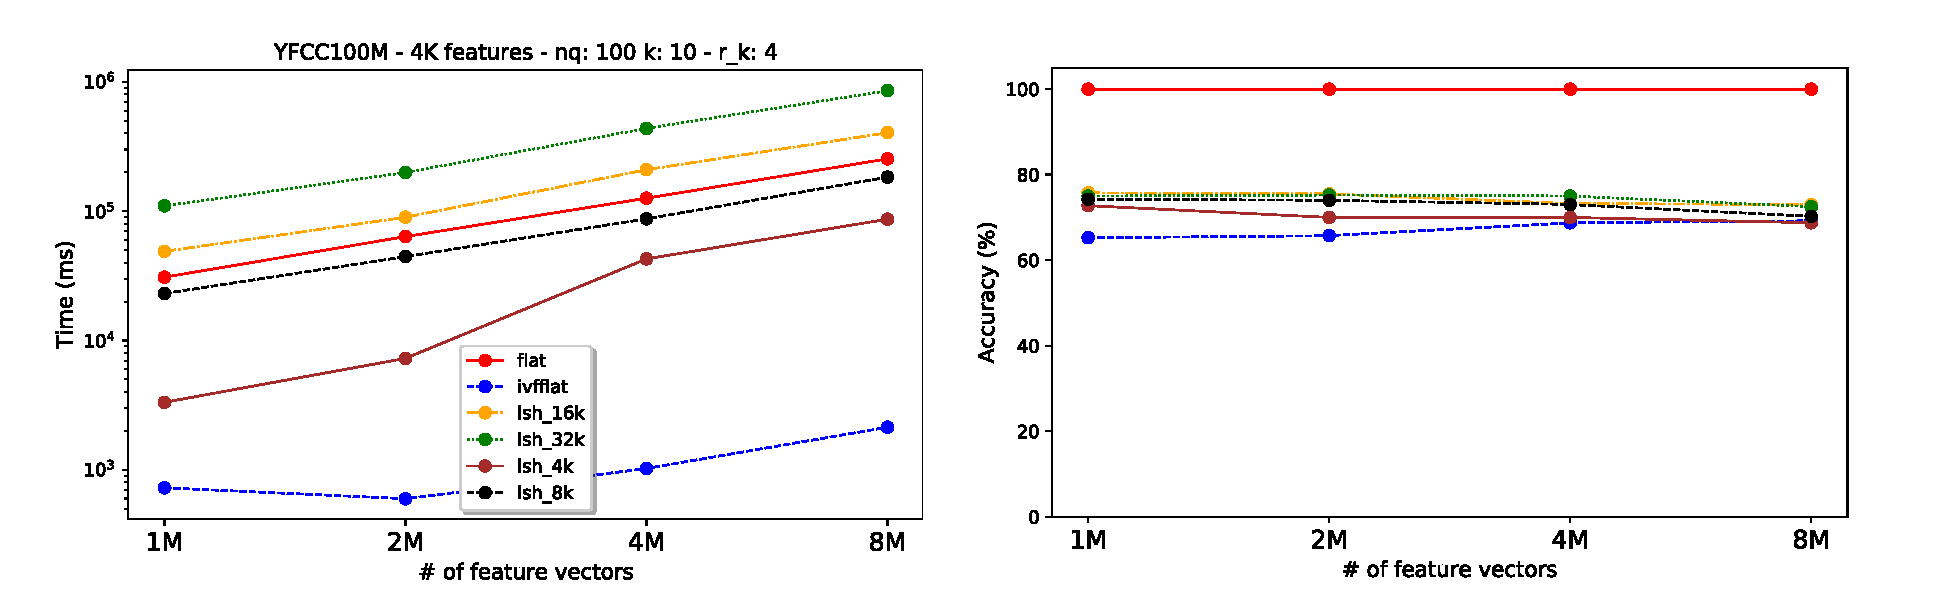
\includegraphics[width=\textwidth]{figures/features_alternatives}
\caption{Feature Vector Evaluation: Trade-off between query execution speed
and accuracy of the results, using ground-truth data for computing accuracy.
For this evaluation, we query the 10 closest neighbors (k = 10), and compute
accuracy using recall at 4 (r\_k = 4) (i.e. percentage of the top 4 ground-truth
results that is present within the top 10 computed neighbors).
We average the query execution time and accuracy for 100 queries (nq = 100).}
\label{fig:features_eval}
\end{figure*}

\begin{figure*}[ht]
\centering
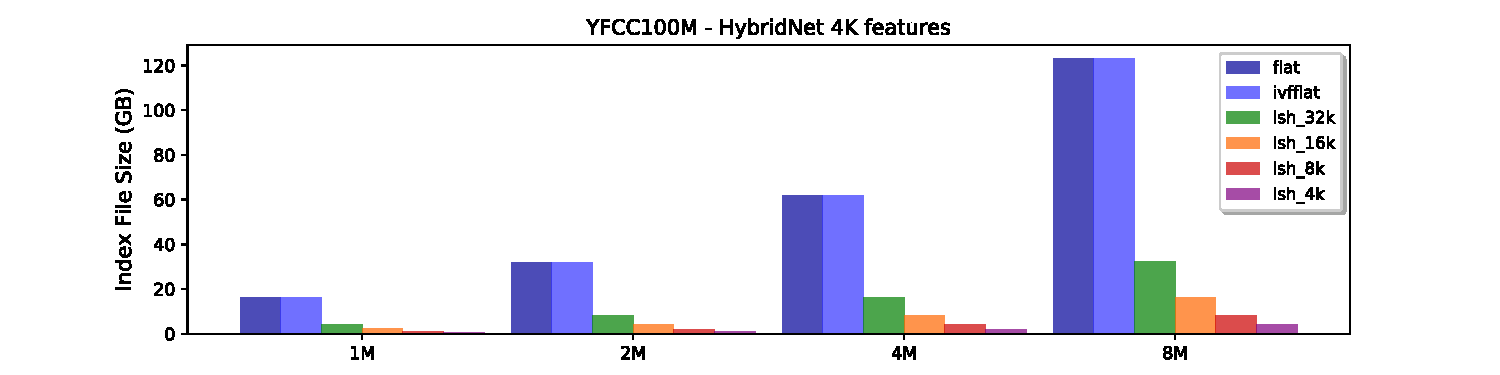
\includegraphics[width=\textwidth]{figures/features_disksize}
\caption{Feature Collection Size in Disk}
\label{fig:features_size_does_matter}
\end{figure*}

As mentioned before, VDMS provides different levels of customization of the
indexes created for a descriptor set, that includes the indexing techniques
and the metric for similarity.
These different indexing techniques come with different trade-offs in terms
of speed of search and accuracy of the computation.
VDMS aims to provide functionality that is agnostics to application-specific
techniques, enabling features that are generic to visual data processing
applications.
Figure~\ref{fig:features_eval} shows an analysis at the different indexing
techniques provided by VDMS and its trades-off between accuracy and query
execution speed, for a single threaded client.
For this evaluation, we query the 10 closest neighbors (k = 10), and compute
accuracy using recall at 4 (r\_k = 4) (i.e. percentage of the top 4 ground-truth
results that is present within the top 10 computed neighbors).
We average the query execution time and accuracy for 100 queries (nq = 100).
The \textit{flat} index (red line) implements exact search and
represents ground-truth, which explain why the
accuracy is always 100\% in the plot on the right.
The other indexes implement \textit{approximate search},
which trades-off between accuracy and speed of search~\cite{flann, faiss}.
We have also tried the \textit{ivfflat} index (inverted file index), as well as
\textit{LSH}-based indexes using a different number of bits per descriptor
\footnote{https://github.com/facebookresearch/faiss/wiki/Faiss-indexes}.
Results show how \textit{ivfflat} is the fastest option but it comes with a trade-off
of about 30\% loss in accuracy, while simple brute-force search
is among the slowest options at the expenses of 100\% accuracy,
meaning exact search.

Another important trade-off to be made is with respect to space efficiency:
The DescriptorSet can grow very large and expensive to load and manage.
In this particular case, 4096-dimensional descriptors for 100M elements
translates into 1TB of data, only in raw floating-point data alone
(without accounting for any metadata or indexes associated with it).
This component is very important for the overall analysis on which
index structure to use because a large set of descriptors may not fit in memory
and thus cause a pressure on the IO system while retrieving descriptors
for computing distance.
This can severely impact the overall query execution time.
When the DescriptorSet grows significantly large,
it may be worth trading off accuracy for speed and space.
Figure~\ref{fig:features_size_does_matter} shows the different indexes and
their size in disk. These indexes already contain all the descriptors (or
a quantized version of them in the case of LSH~\cite{lsh}),
and can be loaded in memory directly when it fits.
Note how, because of quantization of the descriptors, \textit{LSH} provides a
significantly lower space foot print, which can be a great option for
large collections of descriptors when accuracy is not a main factor.
It is not uncommon to sacrifice accuracy as images and videos are captured
using a noise sensor (i.e., the camera), and an approximate search
in many cases can provide the necessary accuracy for applications
to achieve their goals.


% \section{APPENDIX - API Samples}

% \begin{appendix}

% \begin{listing}[ht!]
% \begin{minted}[frame=single,
%               framesep=3mm,
%               linenos=true,
%               xleftmargin=21pt,
%               tabsize=4]{js}
% "FindEntity"{     
%     "class": "autotag",
%     "constraints": { 
%         "name": ["==", "alligator"]
%     }
%     "_ref" : 1
% },
% "FindImage":{
%     "format": "png",
%     "link": {
%         "ref":1,
%         "constraints": {
%             "prob": [">=", 0.66]
%         }
%     }
%     "operations": [{
%         "type": "resize",
%         "height": 224,
%         "width":  224,
%     }]
% }

% \end{minted}
% \caption{Sample Query for Images - 
% The query expresses the following: 
% Find all the images connected to the autotag \textit{alligator} 
% with probability higher than 0.66, apply a resize operation
% to make the images 224x224, and convert to "png".} 
% \label{findimage}
% \end{listing}

% \begin{listing}[t!]
% \begin{minted}[frame=single,
%               framesep=3mm,
%               linenos=true,
%               xleftmargin=21pt,
%               tabsize=4]{js}
% "FindEntity"{     
%     "class": "autotag",
%     "constraints": { 
%         "name": ["==", "alligator"]
%     }
%     "_ref" : 1
% },
% "FindImage":{
%     "format": "png",
%     "link": {
%         "ref":1,
%         "constraints": {
%             "prob": [">=", 0.66]
%         }
%     }, 
%     "constraints": {
%         "latitude": [">=", 36.23433, 
%                      "<=", 38.23433]
%         "longitude":[">=", -114.80666, 
%                      "<=", -116.80666]
%     },
%     "operations": [{
%         "type": "resize",
%         "height": 224,
%         "width":  224,
%     }, {
%         "type": "rotate",
%         "angle": 45.34
%     }]
% }

% \end{minted}
% \caption{Sample Query for Images - 
% The query expresses the following: 
% Find all the images connected to the autotag \textit{alligator} 
% with probability higher than 0.66, 
% filter by latitude and longitude within 1 degree, 
% apply a resize operation to make the images 224x224
% and rotate the image 45.34 degrees, 
% and return the images as "png" files.} 
% \label{findimagegeo}
% \end{listing}

% \end{appendix}


% \section{Final Thoughts on Good Layout}
% Please use readable font sizes in the figures and graphs. Avoid tempering with the correct border values, and the spacing (and format) of both text and captions of the PVLDB format (e.g. captions are bold).

% At the end, please check for an overall pleasant layout, e.g. by ensuring a readable and logical positioning of any floating figures and tables. Please also check for any line overflows, which are only allowed in extraordinary circumstances (such as wide formulas or URLs where a line wrap would be counterintuitive).

% Use the \texttt{balance} package together with a \texttt{\char'134 balance} command at the end of your document to ensure that the last page has balanced (i.e. same length) columns.

\end{document}
